%! Author = crist
%! Date = 25/10/2026

\spacing{1.3}
%----------------------------------------------------------------------------------------
%	UNIDAD 3: EL ENLACE QUÍMICO (4.º ESO)
%   Figuras: images/UD3/*.pdf (fuente HTML en images/UD3/html, SVG en images/UD3/svg)
%----------------------------------------------------------------------------------------

%------------------------------------------------
% Comandos propios de la unidad
%------------------------------------------------
% Configuración electrónica en letra recta (también definido en la UD2)
\providecommand{\conf}[1]{\(\mathrm{#1}\)}
% Diagramas de Lewis con chemfig: \chemfig{H-\charge{90=\:,0=\:,270=\:}{Cl}}
%   \. = un electrón, \: = un par; ángulos 0 (dcha.), 90 (arriba), 180 (izda.), 270 (abajo)
% Corchetes para los iones en los diagramas de Lewis: \ionlewis{\chemfig{...}}{-}
\providecommand{\ionlewis}[2]{\(\Bigl[\)\,#1\,\(\Bigr]^{#2}\)}
% Puntos de Lewis más separados del símbolo y en rojo (como en las figuras)
\setcharge{extra sep=2pt, .radius=0.22ex, :sep=0.45em, .style={fill=red!75!black}}

% Mapa conceptual del tema (fuente en images/mapas_conceptuales/html/temas.js)
\begin{figure}[H]
    \centering
    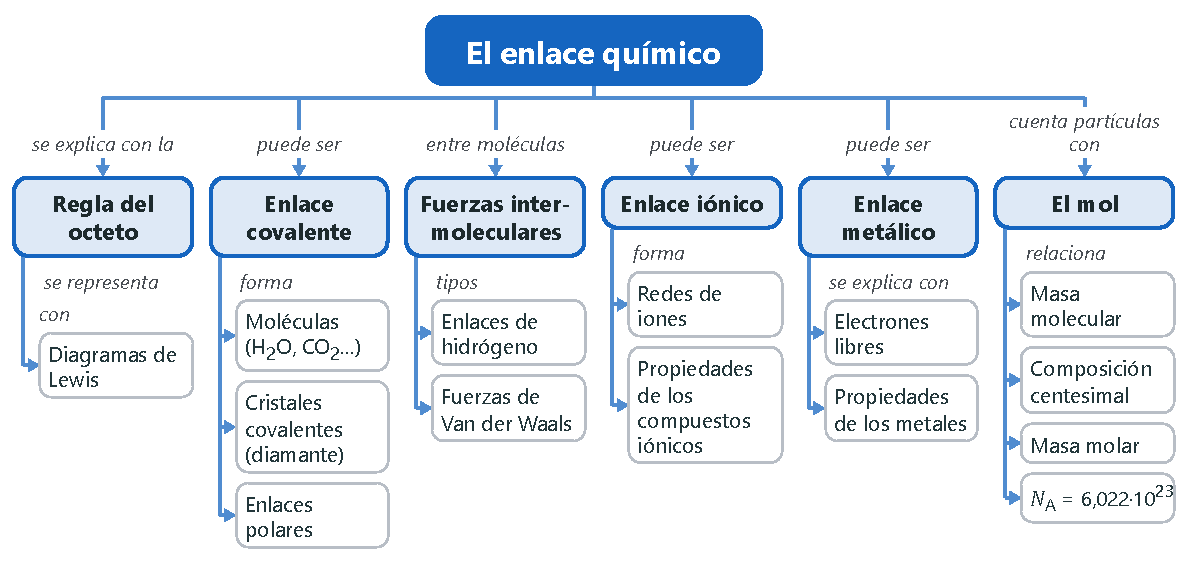
\includegraphics[width=\textwidth]{images/mapas_conceptuales/mapa_UD3}
\end{figure}

%========================================================================================
%\section*{Para empezar: las formas alotrópicas del carbono}
%\addcontentsline{toc}{section}{Para empezar: las formas alotrópicas del carbono}
%========================================================================================
%
%Hablamos de \textbf{alotropía} cuando un mismo elemento, en el mismo estado físico, se presenta en variedades distintas con propiedades físicas y químicas diferentes. Le ocurre a muchos metales y no metales, pero el ejemplo más famoso es el carbono. En la naturaleza aparece como \textbf{grafito} (la mina de los lápices) y como \textbf{diamante}, y en el laboratorio se han obtenido otras formas sorprendentes (figura~\ref{fig:alotropos_carbono}):
%
%\begin{itemize}
%    \item Los \textbf{fullerenos} son «jaulas» de entre 28 y \num{1500} átomos de carbono. Los más conocidos son las \emph{bucky balls}, esferas de 60 átomos con forma de balón de fútbol. Los \textbf{nanotubos} también son fullerenos, con forma de tubo. Tienen propiedades semiconductoras y superconductoras, por lo que interesan a las industrias electrónica, óptica y biomédica; además, por su forma y por ser compatibles con el organismo, pueden transportar fármacos dentro del cuerpo.
%    \item El \textbf{grafeno} es una lámina plana de átomos de carbono colocados en forma de panal de abejas. Como tiene solo un átomo de espesor, se considera un material \textbf{bidimensional}. Es transparente y conduce el calor y la electricidad mejor que el silicio, por lo que podría sustituirlo en la electrónica del futuro.
%\end{itemize}
%
%\begin{figure}[H]
%    \centering
%    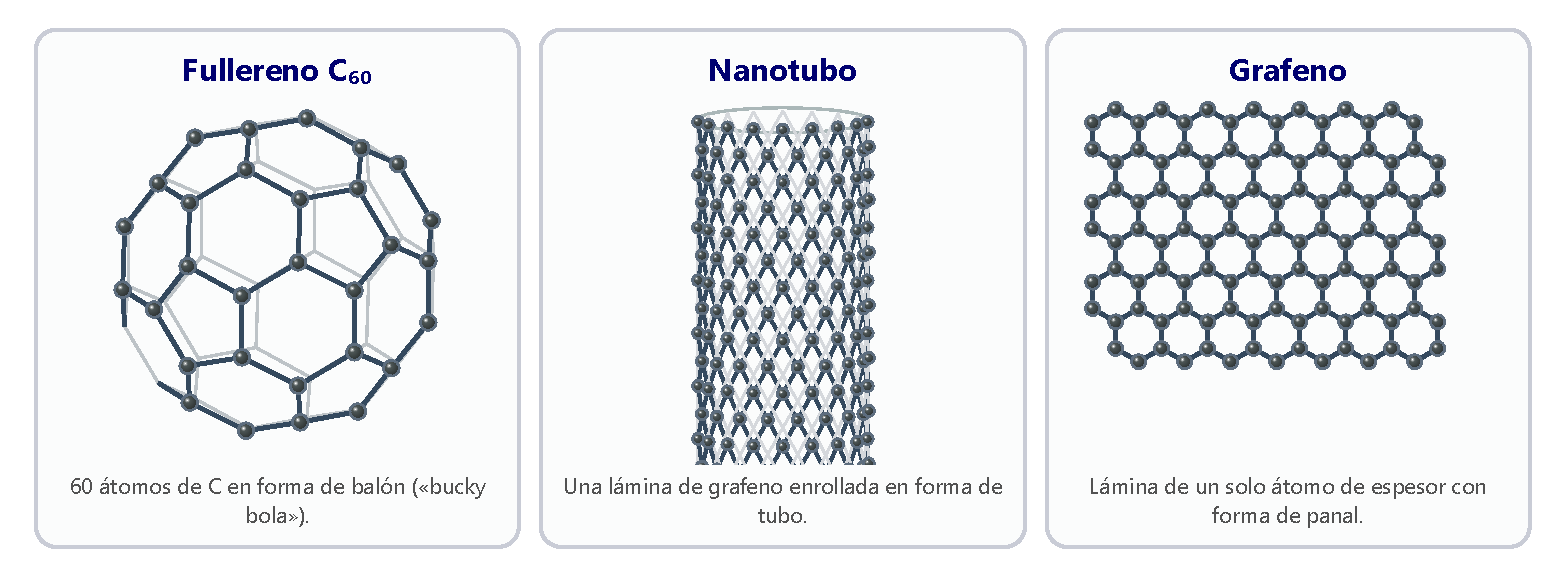
\includegraphics[width=\textwidth]{images/UD3/alotropos_carbono}
%    \caption{Algunas formas alotrópicas del carbono obtenidas en el laboratorio.}
%    \label{fig:alotropos_carbono}
%\end{figure}
%
%\begin{remark}
%    \textbf{Carbono y Objetivos de Desarrollo Sostenible.} Los fullerenos se usan en la industria farmacéutica para transportar medicamentos (\textbf{ODS 3}, \emph{Salud y bienestar}), y el grafeno se investiga para fabricar dispositivos electrónicos y gestionar mejor la energía (\textbf{ODS 7}, \emph{Energía asequible y no contaminante}). Al ser el carbono un elemento muy abundante, su uso no tiene por qué amenazar los recursos naturales.
%\end{remark}
%
%\begin{exercise}
%    Explica con tus palabras qué es la alotropía. ¿Qué formas alotrópicas del carbono se encuentran en la naturaleza y cuáles se han fabricado en el laboratorio?
%    \begin{solu}
%        La alotropía es la existencia de variedades distintas de un mismo elemento, en el mismo estado físico, con propiedades físicas y químicas diferentes. En la naturaleza el carbono aparece como \textcolor{red}{grafito y diamante}; en el laboratorio se han obtenido los \textcolor{red}{fullerenos} (como las \emph{bucky balls}), los \textcolor{red}{nanotubos} y el \textcolor{red}{grafeno}.
%    \end{solu}
%\end{exercise}
%
%\begin{exercise}
%    ¿Cuántos átomos forman los fullerenos? ¿Por qué resultan útiles en medicina? ¿Y en la industria electrónica y óptica?
%    \begin{solu}
%        Están formados por entre 28 y \num{1500} átomos de carbono. Por su estructura y su biocompatibilidad pueden \textcolor{red}{transportar fármacos} dentro del organismo. En electrónica y óptica interesan porque tienen propiedades \textcolor{red}{semiconductoras y superconductoras}.
%    \end{solu}
%\end{exercise}
%
%\begin{exercise}
%    ¿Qué es el grafeno? ¿Por qué se dice que es un material bidimensional? ¿Qué propiedad lo convierte en candidato para sustituir al silicio?
%    \begin{solu}
%        Es una lámina plana de átomos de carbono dispuestos en forma de panal. Es bidimensional porque tiene \textcolor{red}{un solo átomo de espesor}. Podría sustituir al silicio porque su \textcolor{red}{conductividad eléctrica es mayor} (y además es transparente).
%    \end{solu}
%\end{exercise}
%
%\begin{exercise}
%    ¿Crees que el uso de las formas alotrópicas del carbono supone una amenaza para el medioambiente? ¿Con qué Objetivos de Desarrollo Sostenible se relacionan?
%    \begin{solu}
%        En principio no, porque el carbono es un elemento abundante y sus aplicaciones no tienen por qué dañar el medio natural. Se relacionan con el \textcolor{red}{ODS 3} (transporte de fármacos) y con el \textcolor{red}{ODS 7} (electrónica y gestión de la energía).
%    \end{solu}
%\end{exercise}

%========================================================================================
\section{¿Por qué se unen los átomos? El enlace químico}
%========================================================================================

¿Por qué el helio o el neón se encuentran en la naturaleza como átomos sueltos, mientras que el oxígeno aparece en forma de moléculas, \ch{O2}? La respuesta está en los \textbf{electrones del último nivel}.

Los gases nobles tienen su último nivel \textbf{completo}: ocho electrones, con configuración \conf{ns^2~np^6}, salvo el helio, que tiene dos (\conf{1s^2}). Esta es la configuración electrónica más estable posible, por eso los gases nobles no se combinan de forma natural con otros elementos y aparecen como \textbf{átomos aislados}. El resto de los elementos se unen entre sí para conseguir una configuración como la del gas noble más próximo en la tabla periódica: esto explica su comportamiento químico.

\subsection{Los diagramas de Lewis y la regla del octeto}

\begin{definition}[Diagrama de Lewis]
    El \textbf{diagrama de Lewis} de un átomo es una forma de representar sus \textbf{electrones de valencia}, es decir, los de su último nivel. Se escribe el símbolo del elemento rodeado de tantos puntos (o aspas) como electrones de valencia tiene.
\end{definition}

\begin{figure}[H]
    \centering
    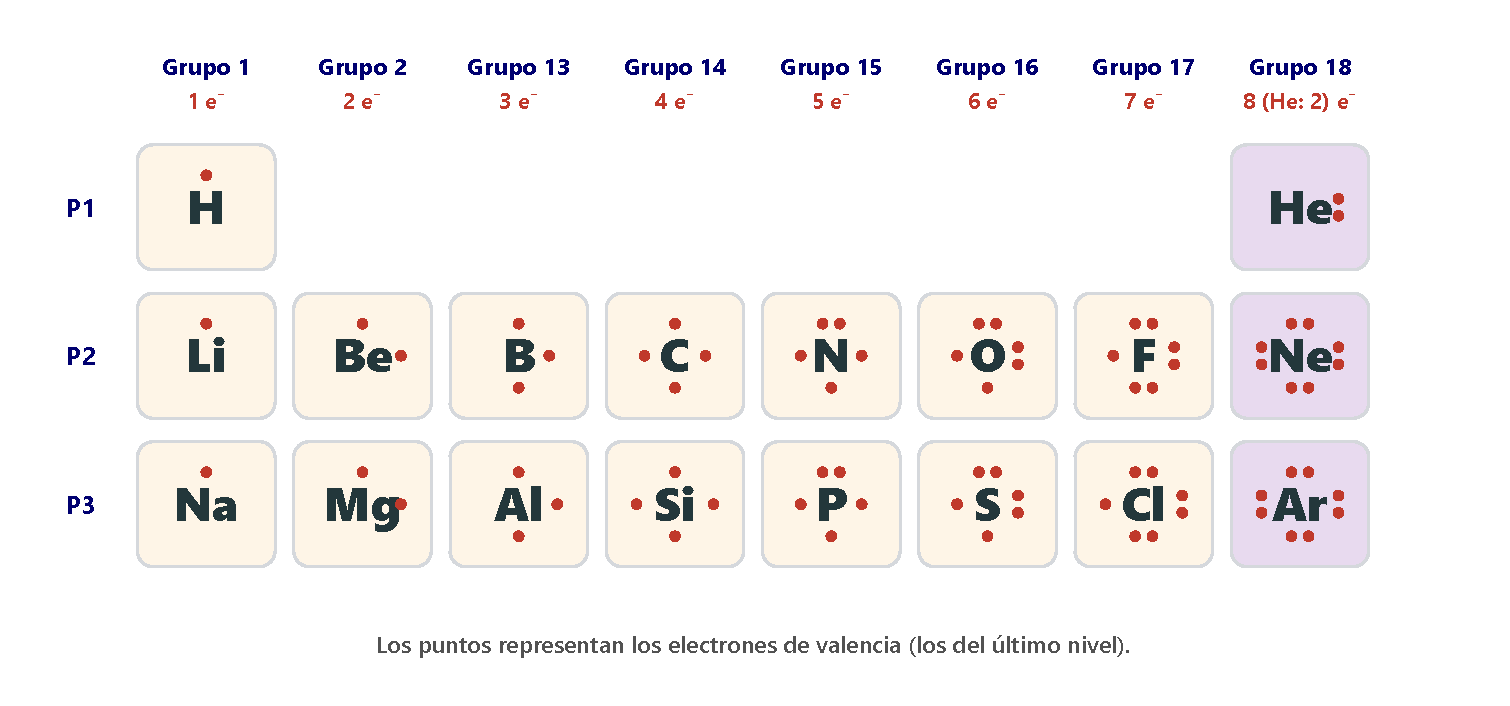
\includegraphics[width=0.9\textwidth]{images/UD3/lewis_tabla}
    \caption{Diagramas de Lewis de los elementos representativos de los tres primeros períodos.}
    \label{fig:lewis_tabla}
\end{figure}

En la figura~\ref{fig:lewis_tabla} se ve, por ejemplo, que al oxígeno le faltan \textbf{dos electrones} para tener ocho, como el neón, mientras que si el litio \textbf{pierde un electrón} se queda con la configuración del helio.

\begin{definition}[Regla del octeto]
    Los átomos tienden a ganar, perder o compartir electrones hasta tener \textbf{ocho electrones en su último nivel} (dos en el caso de los que se acercan al helio), igual que los gases nobles. Esta regla se cumple, sobre todo, en los elementos representativos.
\end{definition}

\begin{exercise}
    Investiga sobre las propiedades físicas y químicas de los gases nobles. ¿Por qué se presentan en la naturaleza como átomos aislados?
    \begin{solu}
        Respuesta libre. Son gases incoloros e inodoros, con puntos de fusión y ebullición muy bajos, y prácticamente no reaccionan con otras sustancias. Se presentan como átomos aislados porque su \textcolor{red}{último nivel está completo} (ocho electrones, o dos en el helio), que es la configuración más estable.
    \end{solu}
\end{exercise}

\begin{exercise}
    Dibuja los diagramas de Lewis de estos elementos: Mg (\(Z = 12\)), Al (\(Z = 13\)), Si (\(Z = 14\)), P (\(Z = 15\)), S (\(Z = 16\)) y Cl (\(Z = 17\)).
    \begin{solu}
        \textcolor{blue}{Todos están en el período 3; sus electrones de valencia son los del nivel 3 (2, 3, 4, 5, 6 y 7, respectivamente):}
        \begin{center}
            \chemfig{\charge{90=\.,0=\.}{Mg}} \qquad
            \chemfig{\charge{90=\.,0=\.,270=\.}{Al}} \qquad
            \chemfig{\charge{90=\.,0=\.,270=\.,180=\.}{Si}} \qquad
            \chemfig{\charge{90=\:,0=\.,270=\.,180=\.}{P}} \qquad
            \chemfig{\charge{90=\:,0=\:,270=\.,180=\.}{S}} \qquad
            \chemfig{\charge{90=\:,0=\:,270=\:,180=\.}{Cl}}
        \end{center}
    \end{solu}
\end{exercise}

\begin{exercise}
    Según la regla del octeto, ¿cuántos electrones tiende a ganar o perder un átomo de\ldots
    \begin{enumerate}[label=\alph*)]
        \item nitrógeno?
        \item un elemento del grupo 17?
        \item calcio?
        \item aluminio?
    \end{enumerate}
    \begin{solu}
        a) El N tiene 5 electrones de valencia: tiende a \textcolor{red}{ganar 3}. b) Tiene 7: tiende a \textcolor{red}{ganar 1}. c) El Ca (grupo 2) tiene 2: tiende a \textcolor{red}{perder 2}. d) El Al (grupo 13) tiene 3: tiende a \textcolor{red}{perder 3}.
    \end{solu}
\end{exercise}

\begin{exercise}
    Haz una tabla con el número de electrones de valencia y el diagrama de Lewis de los elementos del período 2: Li, Be, B, C, N, O, F y Ne.
    \begin{solu}
        \begin{center}
            % --- tabla antigua ---
            % \begin{tblr}{colspec={lcccccccc}, hlines, vlines, row{1}={bg=ocre!85, fg=white, font=\bfseries}, cell{1}{1}={bg=ocre!85, fg=white}}
                % Elemento & Li & Be & B & C & N & O & F & Ne \\
                % Electrones de valencia & 1 & 2 & 3 & 4 & 5 & 6 & 7 & 8 \\
                % Lewis & \chemfig{\charge{90=\.}{Li}} & \chemfig{\charge{90=\.,0=\.}{Be}} & \chemfig{\charge{90=\.,0=\.,270=\.}{B}} & \chemfig{\charge{90=\.,0=\.,270=\.,180=\.}{C}} & \chemfig{\charge{90=\:,0=\.,270=\.,180=\.}{N}} & \chemfig{\charge{90=\:,0=\:,270=\.,180=\.}{O}} & \chemfig{\charge{90=\:,0=\:,270=\:,180=\.}{F}} & \chemfig{\charge{90=\:,0=\:,270=\:,180=\:}{Ne}} \\
            % \end{tblr}
            % --- tabla nueva ---
            \begin{tabular}{@{}lcccccccc@{}}
                \toprule
                \textbf{Elemento} & \textbf{Li} & \textbf{Be} & \textbf{B} & \textbf{C} & \textbf{N} & \textbf{O} & \textbf{F} & \textbf{Ne} \\
                \midrule
                Electrones de valencia & 1 & 2 & 3 & 4 & 5 & 6 & 7 & 8 \\[3pt]
                Lewis & \chemfig{\charge{90=\.}{Li}} & \chemfig{\charge{90=\.,0=\.}{Be}} & \chemfig{\charge{90=\.,0=\.,270=\.}{B}} & \chemfig{\charge{90=\.,0=\.,270=\.,180=\.}{C}} & \chemfig{\charge{90=\:,0=\.,270=\.,180=\.}{N}} & \chemfig{\charge{90=\:,0=\:,270=\.,180=\.}{O}} & \chemfig{\charge{90=\:,0=\:,270=\:,180=\.}{F}} & \chemfig{\charge{90=\:,0=\:,270=\:,180=\:}{Ne}} \\
                \bottomrule
            \end{tabular}
        \end{center}
    \end{solu}
\end{exercise}

\begin{exercise}
    Escribe la configuración electrónica y el diagrama de Lewis del potasio (\(Z = 19\)). ¿Le resulta más fácil alcanzar la configuración de un gas noble ganando o perdiendo electrones? ¿De qué gas noble se trata?
    \begin{solu}
        K: \conf{1s^2~2s^2~2p^6~3s^2~3p^6~4s^1}; Lewis: \chemfig{\charge{90=\.}{K}}. Tiene un solo electrón de valencia, así que le resulta mucho más fácil \textcolor{red}{perderlo} que ganar siete. Así adquiere la configuración del \textcolor{red}{argón}.
    \end{solu}
\end{exercise}

\begin{exercise}
    Indica si son verdaderas o falsas estas afirmaciones y corrige las falsas:
    \begin{enumerate}[label=\alph*)]
        \item Todos los gases nobles tienen ocho electrones en su último nivel.
        \item Hay un elemento del grupo 18 con solo dos electrones en su último nivel.
        \item Algunos gases nobles son sólidos a temperatura ambiente.
        \item Los gases nobles se encuentran en la naturaleza como átomos aislados.
    \end{enumerate}
    \begin{solu}
        a) \textcolor{red}{Falsa}: todos tienen ocho, salvo el helio, que tiene dos. b) \textcolor{red}{Verdadera}: el helio. c) \textcolor{red}{Falsa}: todos los elementos del grupo 18 son gases a temperatura ambiente. d) \textcolor{red}{Verdadera}.
    \end{solu}
\end{exercise}

\begin{exercise}
    Un compañero ha dibujado estos diagramas de Lewis de átomos en su estado fundamental. ¿Cuáles son incorrectos? Escríbelos todos correctamente.
    \begin{center}
        \chemfig{\charge{90=\.,0=\.,180=\.}{Ca}} \qquad
        \chemfig{\charge{90=\:,0=\.,270=\.}{O}} \qquad
        \chemfig{\charge{90=\.,0=\.,270=\.,180=\.}{C}} \qquad
        \chemfig{\charge{90=\:,0=\:,270=\:}{Cl}} \qquad
        \chemfig{\charge{90=\:,0=\.,270=\.,180=\.}{N}}
    \end{center}
    \begin{solu}
        \textcolor{blue}{Contamos los electrones de valencia: Ca 2, O 6, C 4, Cl 7, N 5.} Son incorrectos los del \textcolor{red}{calcio} (tiene 3 puntos en lugar de 2), el \textcolor{red}{oxígeno} (4 en lugar de 6) y el \textcolor{red}{cloro} (6 en lugar de 7). Los correctos son:
        \begin{center}
            \chemfig{\charge{90=\.,0=\.}{Ca}} \qquad
            \chemfig{\charge{90=\:,0=\:,270=\.,180=\.}{O}} \qquad
            \chemfig{\charge{90=\.,0=\.,270=\.,180=\.}{C}} \qquad
            \chemfig{\charge{90=\:,0=\:,270=\:,180=\.}{Cl}} \qquad
            \chemfig{\charge{90=\:,0=\.,270=\.,180=\.}{N}}
        \end{center}
    \end{solu}
\end{exercise}

\subsection{¿Qué es un enlace químico?}

\begin{definition}[Enlace químico]
    Un \textbf{enlace químico} es la fuerza de tipo \textbf{electrostático} que mantiene unidos a los átomos en un elemento o en un compuesto.
\end{definition}

Veámoslo con la molécula más sencilla, la de hidrógeno, \ch{H2} (figura~\ref{fig:fuerzas_h2}). Cuando dos átomos de hidrógeno se acercan aparecen varias fuerzas:

\begin{itemize}
    \item Los dos \textbf{núcleos}, ambos positivos, \textbf{se repelen}.
    \item Los dos \textbf{electrones}, ambos negativos, también \textbf{se repelen}.
    \item Cada núcleo \textbf{atrae} a los dos electrones (el suyo y el del otro átomo).
\end{itemize}

El enlace se forma cuando las fuerzas de \textbf{atracción} superan a las de \textbf{repulsión}: los átomos quedan unidos a una distancia en la que el sistema es más estable que cuando estaban separados.

\begin{figure}[H]
    \centering
    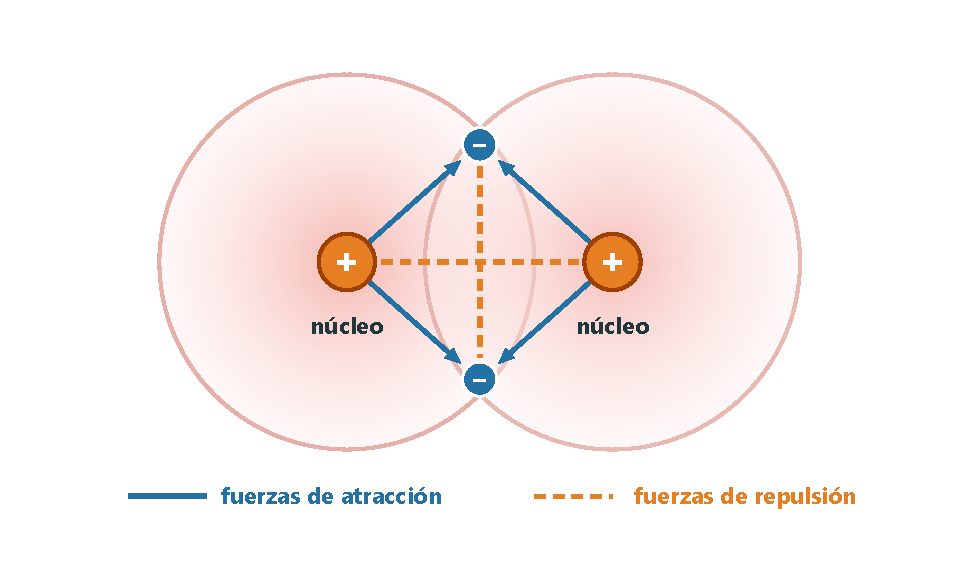
\includegraphics[width=0.55\textwidth]{images/UD3/fuerzas_h2}
    \caption{Fuerzas de atracción y de repulsión entre los núcleos y los electrones de dos átomos de hidrógeno.}
    \label{fig:fuerzas_h2}
\end{figure}

\begin{exercise}
    Define con tus palabras qué es un enlace químico.
    \begin{solu}
        Es la \textcolor{red}{fuerza de tipo electrostático} que mantiene unidos a los átomos dentro de un elemento o de un compuesto.
    \end{solu}
\end{exercise}

\begin{exercise}
    Haz en tu cuaderno un esquema de dos átomos de hidrógeno unidos y señala en él todas las fuerzas de atracción y de repulsión entre núcleos y electrones. ¿Qué condición se tiene que cumplir para que se forme el enlace?
    \begin{solu}
        Como en la figura~\ref{fig:fuerzas_h2}: \textcolor{blue}{repulsión} núcleo--núcleo y electrón--electrón; \textcolor{blue}{atracción} de cada núcleo sobre los dos electrones. El enlace se forma cuando las \textcolor{red}{fuerzas de atracción contrarrestan a las de repulsión}.
    \end{solu}
\end{exercise}

%========================================================================================
\section{El enlace covalente en elementos y compuestos}
%========================================================================================

\begin{definition}[Enlace covalente]
    Los átomos que consiguen su estabilidad \textbf{compartiendo electrones} con otros átomos están unidos mediante \textbf{enlaces covalentes}. Se da entre átomos de \textbf{no metales}. Cada par de electrones compartidos es un enlace.
\end{definition}

\subsection{Elementos covalentes moleculares}

El hidrógeno, el nitrógeno, el oxígeno y los halógenos (flúor, cloro, bromo y yodo) forman \textbf{moléculas diatómicas}: \ch{H2}, \ch{N2}, \ch{O2}, \ch{F2}, \ch{Cl2}, \ch{Br2}, \ch{I2}. Otros, como el fósforo (\ch{P4}) o el azufre (\ch{S8}), forman moléculas de más átomos. Según los electrones que compartan, el enlace puede ser sencillo, doble o triple (figura~\ref{fig:enlaces_f2_o2_n2}):

\begin{itemize}
    \item \textbf{Flúor, \ch{F2}: enlace sencillo.} Cada átomo de flúor (\conf{1s^2~2s^2~2p^5}) tiene 7 electrones de valencia y le falta uno. Los dos átomos comparten \textbf{un par} de electrones y cada uno queda rodeado de ocho.
    \item \textbf{Oxígeno, \ch{O2}: enlace doble.} Cada oxígeno (\conf{1s^2~2s^2~2p^4}) tiene 6 electrones de valencia y le faltan dos, así que los átomos comparten \textbf{dos pares}.
    \item \textbf{Nitrógeno, \ch{N2}: enlace triple.} Cada nitrógeno (\conf{1s^2~2s^2~2p^3}) tiene 5 electrones de valencia y le faltan tres: comparten \textbf{tres pares}.
\end{itemize}

En los tres casos cada átomo acaba rodeado de ocho electrones, como el neón. En las fórmulas desarrolladas cada par compartido se dibuja como un guion: \chemfig{F-F}, \chemfig{O=O}, \chemfig{N~N}.

\begin{figure}[H]
    \centering
    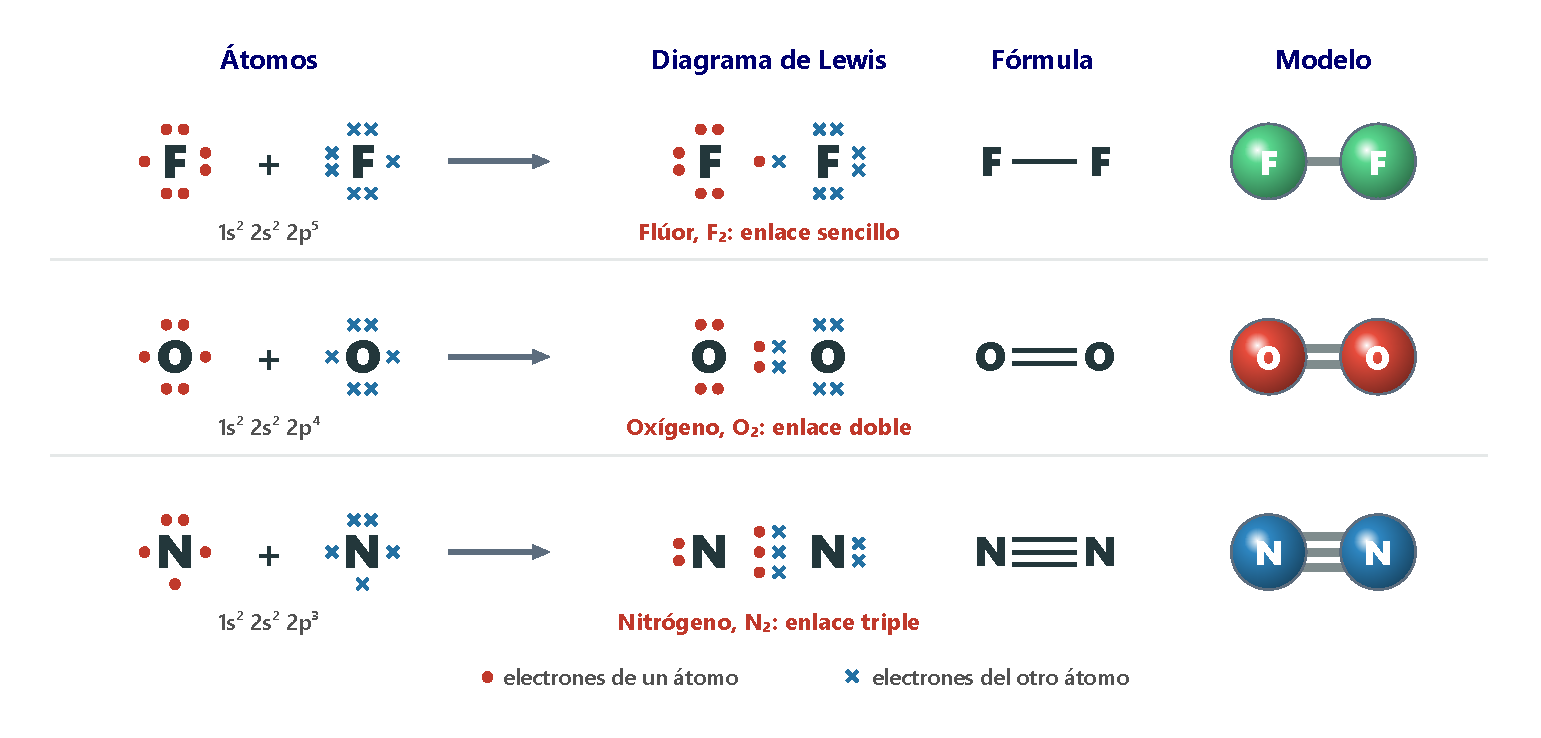
\includegraphics[width=\textwidth]{images/UD3/enlaces_f2_o2_n2}
    \caption{Formación de los enlaces sencillo, doble y triple en las moléculas de flúor, oxígeno y nitrógeno.}
    \label{fig:enlaces_f2_o2_n2}
\end{figure}

\paragraph{Propiedades de los elementos covalentes moleculares.} Suelen ser \textbf{gases} (\ch{H2}, \ch{O2}, \ch{N2}, \ch{F2}, \ch{Cl2}); el bromo es líquido y el yodo es un sólido que sublima con facilidad.
\begin{itemize}
    \item Tienen puntos de fusión y de ebullición \textbf{bajos}.
    \item \textbf{No conducen} la corriente eléctrica, porque no tienen electrones libres.
    \item Son \textbf{insolubles} o muy poco solubles en agua.
\end{itemize}

\begin{exercise}
    Fíjate en la figura~\ref{fig:enlaces_f2_o2_n2} y responde:
    \begin{enumerate}[label=\alph*)]
        \item ¿Cuántos electrones comparten los dos átomos en las moléculas de flúor, de oxígeno y de nitrógeno?
        \item ¿De cuántos electrones queda rodeado cada átomo?
        \item ¿Cuántos enlaces covalentes hay en cada molécula?
        \item ¿A qué gas noble se parecen así?
    \end{enumerate}
    \begin{solu}
        a) \ch{F2}: un par (2 electrones); \ch{O2}: dos pares (4 electrones); \ch{N2}: tres pares (6 electrones). b) De \textcolor{red}{ocho} electrones. c) \ch{F2}: \textcolor{red}{uno}; \ch{O2}: \textcolor{red}{dos}; \ch{N2}: \textcolor{red}{tres}. d) Al \textcolor{red}{neón}.
    \end{solu}
\end{exercise}

\begin{exercise}
    El bromo tiene número atómico \(Z = 35\).
    \begin{enumerate}[label=\alph*)]
        \item Escribe su configuración electrónica. ¿Cuántos electrones tiene en su último nivel?
        \item ¿Qué tipo de molécula forma? ¿Por qué?
        \item Representa con diagramas de Lewis cómo se forma la molécula.
    \end{enumerate}
    \begin{solu}
        a) \conf{1s^2~2s^2~2p^6~3s^2~3p^6~4s^2~3d^{10}~4p^5}. Tiene \textcolor{red}{7 electrones} en el último nivel (\(4s^2\,4p^5\)).
        b) Le falta un electrón para completar el octeto. Dos átomos de bromo comparten un par de electrones y forman una \textcolor{red}{molécula diatómica, \ch{Br2}}, con un enlace sencillo.
        c)
        \begin{center}
            \chemfig{\charge{90=\:,270=\:,180=\:,0=\.}{Br}} \(\;+\;\) \chemfig{\charge{90=\:,270=\:,0=\:,180=\.}{Br}} \(\;\longrightarrow\;\) \chemfig{\charge{90=\:,270=\:,180=\:}{Br}-\charge{90=\:,270=\:,0=\:}{Br}}
        \end{center}
    \end{solu}
\end{exercise}

\begin{exercise}
    Indica si el enlace entre los átomos de estas moléculas es sencillo, doble o triple: \ch{Cl2}, \ch{N2}, \ch{H2}, \ch{O2}, \ch{I2}. ¿Cuántos pares de electrones se comparten en cada una?
    \begin{solu}
        \ch{Cl2}: \textcolor{red}{sencillo} (1 par); \ch{N2}: \textcolor{red}{triple} (3 pares); \ch{H2}: \textcolor{red}{sencillo} (1 par); \ch{O2}: \textcolor{red}{doble} (2 pares); \ch{I2}: \textcolor{red}{sencillo} (1 par).
    \end{solu}
\end{exercise}

\begin{exercise}
    Dados los no metales neón, hidrógeno, bromo, carbono (diamante), nitrógeno, argón, carbono (grafito), oxígeno y cloro:
    \begin{enumerate}[label=\alph*)]
        \item Clasifícalos según se presenten en la naturaleza como átomos aislados, moléculas diatómicas o cristales covalentes.
        \item En las moléculas diatómicas, indica si el enlace es sencillo, doble o triple.
    \end{enumerate}
    \begin{solu}
        a) Átomos aislados: \textcolor{red}{neón y argón}. Moléculas diatómicas: \textcolor{red}{hidrógeno, bromo, nitrógeno, oxígeno y cloro}. Cristales covalentes: \textcolor{red}{diamante y grafito}.
        b) Sencillo: \ch{H2}, \ch{Br2} y \ch{Cl2}; doble: \ch{O2}; triple: \ch{N2}.
    \end{solu}
\end{exercise}

\subsection{Elementos en forma de cristales covalentes}

El carbono tiene puntos de fusión y ebullición muy altos, tanto en forma de grafito como de diamante, así que no puede estar formado por moléculas pequeñas. El átomo de carbono (\(Z = 6\), \conf{1s^2~2s^2~2p^2}) tiene cuatro electrones de valencia y le faltan cuatro: los consigue compartiendo un electrón con cada uno de \textbf{cuatro átomos de carbono} vecinos. Cada uno de estos, a su vez, se une a otros, y así sucesivamente, hasta formar una \textbf{red cristalina} gigante. A estas sustancias se les llama \textbf{cristales covalentes} o \textbf{sólidos reticulares}.

\begin{figure}[H]
    \centering
    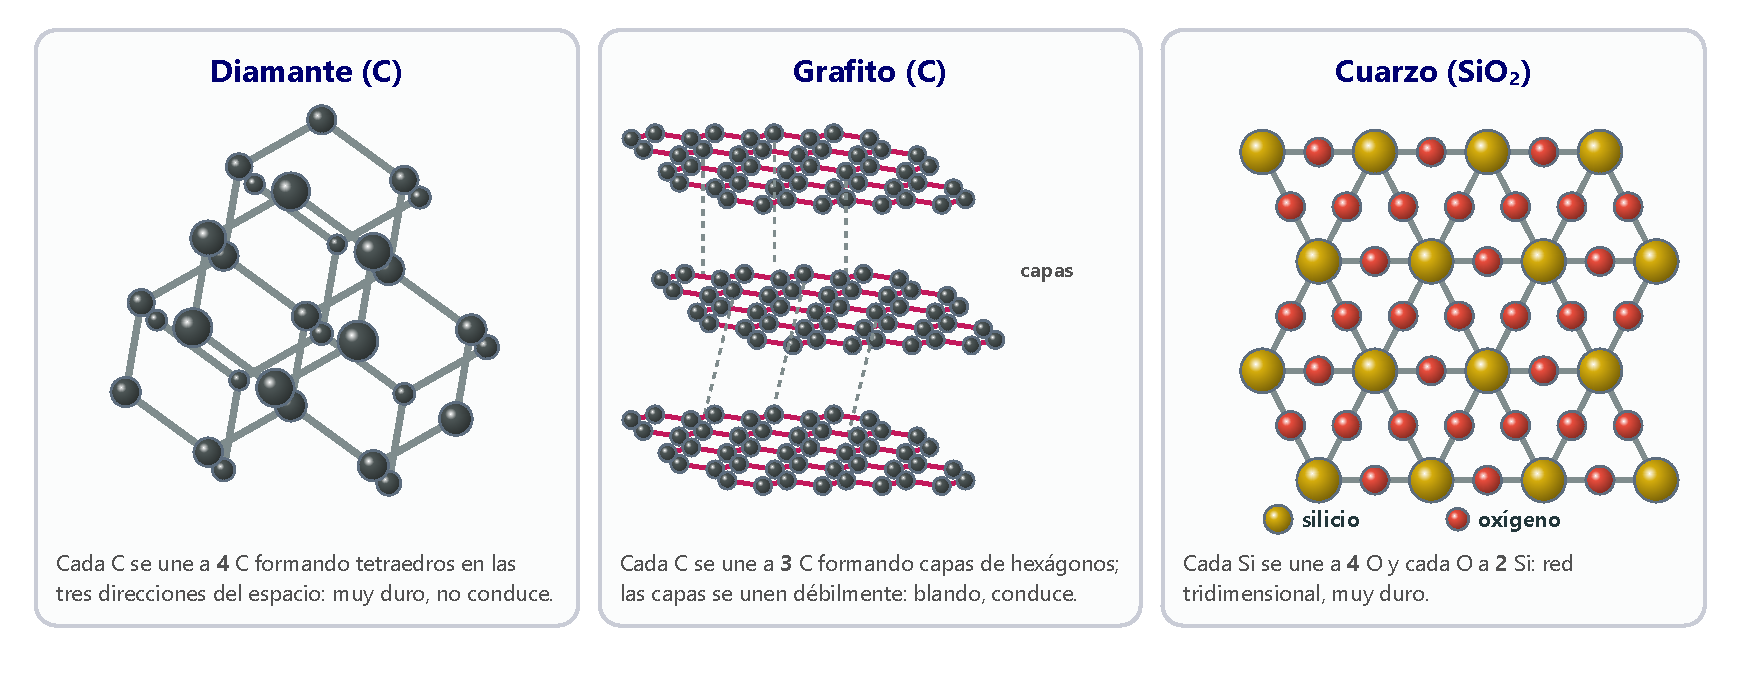
\includegraphics[width=\textwidth]{images/UD3/cristales_covalentes}
    \caption{Estructura de tres cristales covalentes: diamante, grafito y cuarzo.}
    \label{fig:cristales_covalentes}
\end{figure}

\begin{multicols}{2}
    \textbf{Diamante.} Cada átomo de carbono se une a otros \textbf{cuatro} formando tetraedros que se extienden en las tres direcciones del espacio. La red es muy fuerte: es una de las sustancias \textbf{más duras} que se conocen y sigue siendo sólida a temperaturas muy altas. Como todos los electrones están fijos en los enlaces, \textbf{no conduce} la corriente eléctrica.

    \columnbreak
    \textbf{Grafito.} Cada átomo de carbono se une fuertemente a otros \textbf{tres} de su mismo plano formando anillos de seis átomos. Las \textbf{capas} así formadas se unen entre sí débilmente y se deslizan unas sobre otras: el grafito es \textbf{blando}, negro y brillante. El cuarto electrón de cada carbono queda bastante libre, por eso el grafito \textbf{conduce} la electricidad.
\end{multicols}

\begin{exercise}
    ¿En qué se parecen y en qué se diferencian un cristal de diamante y uno de grafito?
    \begin{solu}
        \textcolor{blue}{Analogías:} los dos son cristales covalentes formados solo por átomos de carbono, tienen puntos de fusión muy altos y son insolubles en agua.
        \textcolor{blue}{Diferencias:} en el diamante cada C se une a 4 átomos en una red tridimensional; es muy duro y no conduce la electricidad. En el grafito cada C se une a 3 formando capas débilmente unidas; es blando, se exfolia en láminas y \textcolor{red}{conduce} la electricidad.
    \end{solu}
\end{exercise}

\begin{exercise}
    Los no metales pueden presentarse como átomos aislados, como moléculas o como cristales covalentes. Pon dos ejemplos de cada caso.
    \begin{solu}
        Respuesta libre. Por ejemplo: átomos aislados, \textcolor{red}{helio y argón}; moléculas, \textcolor{red}{\ch{O2} y \ch{Cl2}}; cristales covalentes, \textcolor{red}{diamante y grafito} (o silicio).
    \end{solu}
\end{exercise}

\begin{exercise}
    Dibuja el diagrama de Lewis de un átomo de silicio (\(Z = 14\)). ¿Por qué crees que el silicio forma cristales parecidos a los del diamante?
    \begin{solu}
        \chemfig{\charge{90=\.,0=\.,270=\.,180=\.}{Si}}. Como el carbono, tiene \textcolor{red}{4 electrones de valencia}, de modo que completa su octeto compartiendo un electrón con cada uno de cuatro átomos vecinos, lo que da lugar a una red tridimensional.
    \end{solu}
\end{exercise}

\begin{exercise}
    Indica si cada propiedad corresponde al diamante, al grafito o a los dos:
    \begin{enumerate}[label=\alph*)]
        \item es un cristal covalente;
        \item no conduce la electricidad;
        \item es muy duro;
        \item conduce la corriente eléctrica;
        \item no se disuelve en agua;
        \item es blando.
    \end{enumerate}
    \begin{solu}
        a) \textcolor{red}{Los dos}. b) \textcolor{red}{Diamante}. c) \textcolor{red}{Diamante}. d) \textcolor{red}{Grafito}. e) \textcolor{red}{Los dos}. f) \textcolor{red}{Grafito}.
    \end{solu}
\end{exercise}

\begin{exercise}
    Tanto en la molécula de \ch{H2} como en el diamante los átomos están unidos por enlaces covalentes. ¿Por qué entonces el hidrógeno es un gas y el diamante un sólido muy duro?
    \begin{solu}
        Las moléculas de \ch{H2} son pequeñas y están \textcolor{red}{aisladas} unas de otras (entre ellas apenas hay atracción), por eso es un gas. El diamante es una \textcolor{red}{red gigante} en la que todos los átomos están unidos por enlaces covalentes; para fundirlo habría que romper muchísimos enlaces, por eso es sólido y muy duro.
    \end{solu}
\end{exercise}

\begin{exercise}
    Haz un dibujo de cómo se unen los átomos de carbono en el diamante y en el grafito, y úsalo para explicar por qué el diamante es tan duro mientras que el grafito es blando y se separa en capas.
    \begin{solu}
        Dibujo como el de la figura~\ref{fig:cristales_covalentes}. En el diamante cada carbono está unido a cuatro en las \textcolor{red}{tres direcciones del espacio}: para rayarlo hay que romper enlaces fuertes en todas las direcciones. En el grafito los enlaces fuertes solo están dentro de cada capa; \textcolor{red}{entre capas la unión es débil}, por eso se deslizan y se separan fácilmente.
    \end{solu}
\end{exercise}

\subsection{Compuestos covalentes moleculares}

Los átomos de \textbf{distintos} no metales también se unen compartiendo electrones y forman \textbf{moléculas covalentes}. Son ejemplos el agua, el cloruro de hidrógeno, el amoníaco, el metano, el dióxido de carbono, el butano o el benceno (figura~\ref{fig:moleculas_covalentes}).

\begin{itemize}
    \item \textbf{Cloruro de hidrógeno, \ch{HCl}.} Al cloro (7 electrones de valencia) le falta uno para parecerse al argón y al hidrógeno (1 electrón) le falta otro para parecerse al helio. Comparten un par de electrones y quedan unidos por un \textbf{enlace sencillo}. La molécula es \textbf{lineal}.
    \item \textbf{Amoníaco, \ch{NH3}.} Al nitrógeno (5 electrones de valencia) le faltan tres. Forma tres enlaces sencillos, uno con cada átomo de hidrógeno, y le queda un par de electrones sin compartir. La molécula tiene forma de \textbf{pirámide}.
\end{itemize}

\begin{figure}[H]
    \centering
    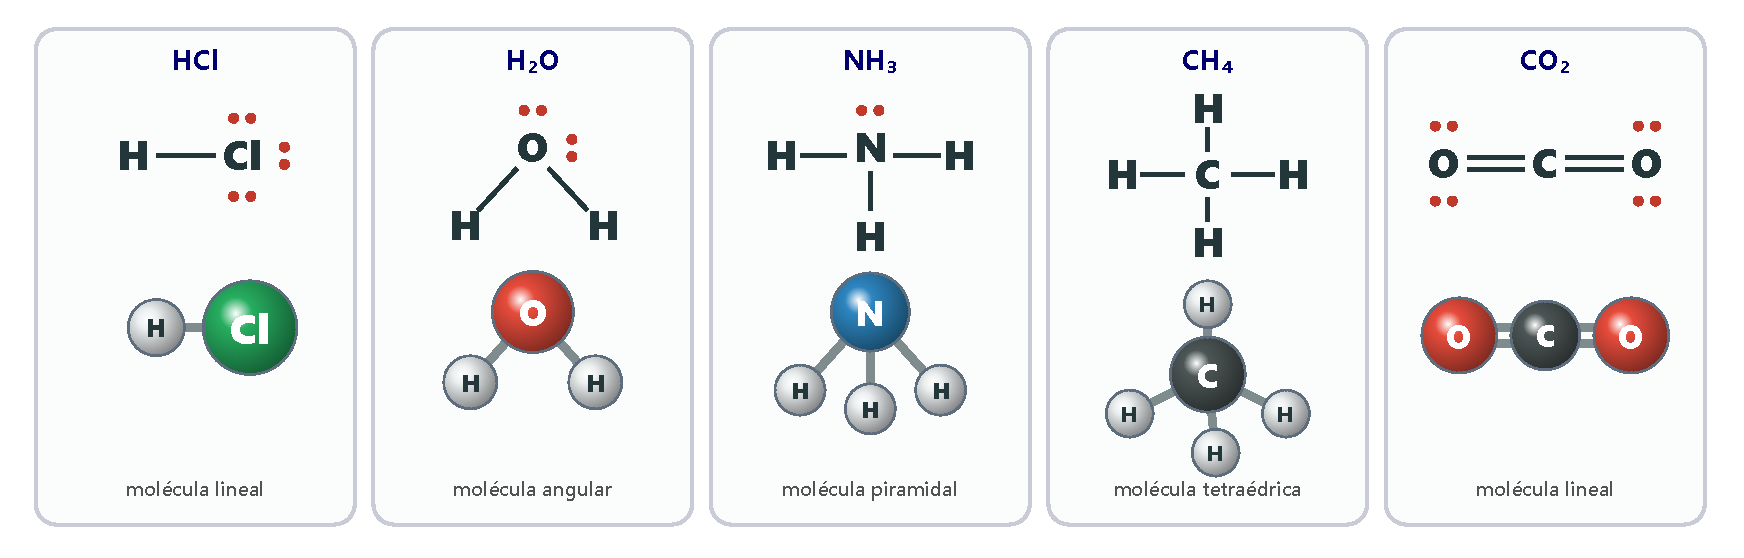
\includegraphics[width=\textwidth]{images/UD3/moleculas_covalentes}
    \caption{Diagramas de Lewis, fórmulas desarrolladas y modelos de bolas de algunas moléculas covalentes. Los puntos rojos son los pares de electrones sin compartir.}
    \label{fig:moleculas_covalentes}
\end{figure}

\paragraph{Propiedades de los compuestos covalentes moleculares.} Pueden ser gases, líquidos o sólidos; los sólidos son frágiles o blandos, como la cera.
\begin{itemize}
    \item Tienen puntos de fusión y ebullición \textbf{bajos}.
    \item Generalmente \textbf{no se disuelven en agua}, pero sí en disolventes como el benceno, el tolueno o la acetona.
    \item \textbf{No conducen} la electricidad.
\end{itemize}

\begin{exercise}
    Observa las propiedades de estas sustancias covalentes moleculares:
    \begin{center}
        % --- tabla antigua ---
        % \begin{tblr}{width=\linewidth, colspec={X[1.3,l]X[c]X[c]X[c]X[1.2,c]X[c]}, cells={font=\small}, hlines, vlines, row{1}={bg=ocre!85, fg=white, font=\small\bfseries}, column{1}={bg=ocre!15, font=\small\bfseries}, cell{1}{1}={bg=ocre!85, fg=white}, rowsep=1pt}
            % & Amoníaco, \ch{NH3} & Metano, \ch{CH4} & Benceno, \ch{C6H6} & Tetracloruro de carbono, \ch{CCl4} & Naftaleno, \ch{C10H8} \\
            % Aspecto & gas incoloro & gas incoloro & líquido incoloro & líquido incoloro & cristales en láminas \\
            % \(T_\text{f}\) (\unit{\celsius}) & \num{-78} & \num{-182} & \num{5.5} & \num{-23} & \num{80} \\
            % \(T_\text{e}\) (\unit{\celsius}) & \num{-33} & \num{-161} & \num{80} & \num{77} & \num{218} \\
            % ¿Conduce? & no & no & no & no & no \\
            % ¿Soluble en agua? & sí & no & no & no & no \\
        % \end{tblr}
        % --- tabla nueva ---
        {\small
        \begin{tabular}{@{}L{0.16\linewidth} c c c C{0.14\linewidth} c@{}}
            \toprule
             & \textbf{Amoníaco, \ch{NH3}} & \textbf{Metano, \ch{CH4}} & \textbf{Benceno, \ch{C6H6}} & \textbf{Tetracloruro de carbono, \ch{CCl4}} & \textbf{Naftaleno, \ch{C10H8}} \\
            \midrule
            \textbf{Aspecto} & gas incoloro & gas incoloro & líquido incoloro & líquido incoloro & cristales en láminas \\[3pt]
            \textbf{\(T_\text{f}\) (\unit{\celsius})} & \num{-78} & \num{-182} & \num{5.5} & \num{-23} & \num{80} \\[3pt]
            \textbf{\(T_\text{e}\) (\unit{\celsius})} & \num{-33} & \num{-161} & \num{80} & \num{77} & \num{218} \\[3pt]
            \textbf{¿Conduce?} & no & no & no & no & no \\[3pt]
            \textbf{¿Soluble en agua?} & sí & no & no & no & no \\
            \bottomrule
        \end{tabular}
        }
    \end{center}
    \begin{enumerate}[label=\alph*)]
        \item ¿Cómo son sus puntos de fusión y ebullición?
        \item ¿En qué estado están a \qty{25}{\celsius}?
        \item ¿Conducen la electricidad?
        \item ¿Son solubles en agua?
        \item ¿Qué propiedades tienen en común?
    \end{enumerate}
    \begin{solu}
        a) Son \textcolor{red}{bajos}. b) A \qty{25}{\celsius}, el amoníaco y el metano son \textcolor{red}{gases} (\(T_\text{e} < \qty{25}{\celsius}\)); el benceno y el tetracloruro de carbono son \textcolor{red}{líquidos} (\(T_\text{f} < \qty{25}{\celsius} < T_\text{e}\)) y el naftaleno es \textcolor{red}{sólido} (\(T_\text{f} > \qty{25}{\celsius}\)). c) \textcolor{red}{No}. d) Salvo el amoníaco, \textcolor{red}{no}. e) Puntos de fusión y ebullición bajos, no conducen la electricidad y casi todas son insolubles en agua.
    \end{solu}
\end{exercise}

\begin{exercise}
    Dibuja los diagramas de Lewis de: \ch{H2}, \ch{HBr}, \ch{F2}, \ch{CH4}, \ch{O2}, \ch{HF}, \ch{H2O}, \ch{NH3} y \ch{H2S}.
    \begin{solu}
        \begin{center}
            \chemfig{H-H} \qquad
            \chemfig{H-\charge{90=\:,0=\:,270=\:}{Br}} \qquad
            \chemfig{\charge{90=\:,180=\:,270=\:}{F}-\charge{90=\:,0=\:,270=\:}{F}} \qquad
            \chemfig{C(-[2]H)(-[4]H)(-[6]H)-H} \qquad
            \chemfig{\charge{90=\:,180=\:}{O}=\charge{90=\:,0=\:}{O}}

            \medskip
            \chemfig{H-\charge{90=\:,0=\:,270=\:}{F}} \qquad
            \chemfig{H-\charge{90=\:,270=\:}{O}-H} \qquad
            \chemfig{H-\charge{90=\:}{N}(-[6]H)-H} \qquad
            \chemfig{H-\charge{90=\:,270=\:}{S}-H}
        \end{center}
    \end{solu}
\end{exercise}

\begin{exercise}
    Interpreta estos diagramas de Lewis: ¿cuántos electrones de valencia tiene cada átomo y qué tipo de enlaces se forman?
    \begin{center}
        \chemfig{\charge{90=\:,270=\:}{O}=C=\charge{90=\:,270=\:}{O}} \qquad
        \chemfig{\charge{180=\:}{N}~\charge{0=\:}{N}} \qquad
        \chemfig{H-\charge{90=\:,270=\:}{Cl}}
    \end{center}
    \begin{solu}
        \textcolor{blue}{\ch{CO2}:} el carbono tiene 4 electrones de valencia y cada oxígeno 6. El carbono comparte dos pares con cada oxígeno: \textcolor{red}{dos enlaces dobles}.
        \textcolor{blue}{\ch{N2}:} cada nitrógeno tiene 5 electrones de valencia y comparte tres con el otro: \textcolor{red}{enlace triple}.
        \textcolor{blue}{\ch{HCl}:} el hidrógeno tiene 1 electrón de valencia y el cloro 7; comparten un par: \textcolor{red}{enlace sencillo}. (Al cloro le quedan tres pares sin compartir: falta uno en el dibujo.)
    \end{solu}
\end{exercise}

\begin{exercise}
    Escribe el diagrama de Lewis del \ch{CO2} y del \ch{N2} sabiendo que \(Z(\ch{C}) = 6\), \(Z(\ch{O}) = 8\) y \(Z(\ch{N}) = 7\).
    \begin{solu}
        \chemfig{\charge{90=\:,270=\:}{O}=C=\charge{90=\:,270=\:}{O}} \qquad \chemfig{\charge{180=\:}{N}~\charge{0=\:}{N}}
    \end{solu}
\end{exercise}

\begin{exercise}
    ¿Por qué se usan los plásticos, que son compuestos covalentes, para recubrir los cables eléctricos?
    \begin{solu}
        Porque los compuestos covalentes moleculares \textcolor{red}{no conducen la corriente eléctrica}: no tienen electrones libres ni iones que puedan moverse. Son buenos aislantes.
    \end{solu}
\end{exercise}

\begin{exercise}
    El sulfuro de hidrógeno, \ch{H2S}, está formado por dos no metales.
    \begin{enumerate}[label=\alph*)]
        \item ¿Qué tipo de enlace hay entre el hidrógeno y el azufre?
        \item ¿Qué propiedades esperas que tenga?
    \end{enumerate}
    \begin{solu}
        a) \textcolor{red}{Covalente}, porque los dos son no metales. b) Será un compuesto molecular: con puntos de fusión y ebullición bajos (de hecho es un gas a temperatura ambiente), poco soluble en agua y \textcolor{red}{no conductor} de la electricidad.
    \end{solu}
\end{exercise}

\begin{exercise}
    El azufre y el oxígeno forman varios compuestos (\ch{SO}, \ch{SO2}, \ch{SO3}), aunque los dos tienen tendencia a captar electrones. ¿Cómo se mantienen unidos sus átomos?
    \begin{solu}
        Como ninguno de los dos cede electrones, los átomos se mantienen unidos \textcolor{red}{compartiendo electrones}: mediante \textcolor{red}{enlaces covalentes}.
    \end{solu}
\end{exercise}

\begin{exercise}
    El germano, \ch{GeH4}, es un gas incoloro que funde a \qty{-165}{\celsius} y hierve a \qty{-88}{\celsius}; no conduce la electricidad y no se disuelve en agua.
    \begin{enumerate}[label=\alph*)]
        \item ¿Qué tipo de enlace tendrá?
        \item ¿Estará formado por moléculas o por cristales?
    \end{enumerate}
    \begin{solu}
        a) Por sus propiedades, el enlace es \textcolor{red}{covalente}. b) Por sus bajísimos puntos de fusión y ebullición, está formado por \textcolor{red}{moléculas}.
    \end{solu}
\end{exercise}

\subsection{Compuestos covalentes en forma de cristales}

Algunos compuestos covalentes, como el \textbf{dióxido de silicio}, \ch{SiO2} (cuarzo, el componente principal de la arena), o el carburo de silicio, \ch{SiC}, son muy duros y tienen puntos de fusión y ebullición muy altos. No están formados por moléculas, sino que son \textbf{redes cristalinas tridimensionales}: en el cuarzo, cada átomo de silicio se une a cuatro de oxígeno y cada oxígeno a dos de silicio (figura~\ref{fig:cristales_covalentes}).

\paragraph{Propiedades de los compuestos covalentes cristalinos.}
\begin{itemize}
    \item Puntos de fusión y ebullición \textbf{muy elevados}: el enlace covalente es muy fuerte y hay que romper muchos enlaces.
    \item Son \textbf{muy duros}: para rayarlos hay que destruir numerosos enlaces covalentes.
    \item \textbf{No conducen} la corriente eléctrica, porque no tienen electrones libres.
    \item \textbf{No se disuelven} en agua ni en otros disolventes.
\end{itemize}

\begin{exercise}
    Indica si cada propiedad corresponde a un compuesto covalente molecular, a uno reticular (cristalino) o a los dos:
    \begin{enumerate}[label=\alph*)]
        \item Puede ser gas, líquido o un sólido blando.
        \item Sólido muy duro.
        \item No conduce la electricidad.
        \item Puntos de fusión y ebullición muy altos.
        \item No se disuelve en agua, pero sí en acetona o tolueno.
        \item No se disuelve en ningún disolvente.
        \item Puntos de fusión y ebullición bajos.
    \end{enumerate}
    \begin{solu}
        a) Molecular. b) Reticular. c) \textcolor{red}{Los dos}. d) Reticular. e) Molecular. f) Reticular. g) Molecular.
    \end{solu}
\end{exercise}

\begin{exercise}
    Dada esta lista de sustancias: carbono (grafito), cuarzo, carbono (diamante), \ch{HBr}, \ch{Cl2}, \ch{Ne}, \ch{HCl}, \ch{Ar}, \ch{I2}, \ch{H2O}, \ch{CH4}, \ch{N2}.
    \begin{enumerate}[label=\alph*)]
        \item Separa los elementos de los compuestos.
        \item Clasifícalas en átomos aislados, moléculas covalentes y cristales covalentes.
        \item Cita dos elementos formados por moléculas diatómicas y dos elementos que no formen moléculas.
        \item Indica una sustancia que conduzca la electricidad y otra que no.
    \end{enumerate}
    \begin{solu}
        a) Elementos: grafito, diamante, \ch{Cl2}, \ch{Ne}, \ch{Ar}, \ch{I2}, \ch{N2}. Compuestos: cuarzo, \ch{HBr}, \ch{HCl}, \ch{H2O}, \ch{CH4}.
        b) Átomos aislados: \ch{Ne}, \ch{Ar}. Moléculas: \ch{HBr}, \ch{Cl2}, \ch{HCl}, \ch{I2}, \ch{H2O}, \ch{CH4}, \ch{N2}. Cristales covalentes: grafito, diamante y cuarzo.
        c) Por ejemplo, \ch{Cl2} y \ch{N2}; \ch{Ne} y el diamante.
        d) Conduce: \textcolor{red}{el grafito}; las demás \textcolor{red}{no conducen} (por ejemplo, el cuarzo).
    \end{solu}
\end{exercise}

\subsection{¿Puede haber cargas eléctricas en un enlace covalente?}

En el enlace covalente los electrones se comparten, pero no siempre a partes iguales:

\begin{itemize}
    \item \textbf{Enlace covalente apolar.} Si los dos átomos son \textbf{iguales} (\ch{Cl2}, \ch{H2}\ldots), atraen por igual a los electrones compartidos. El centro de las cargas positivas (núcleos) coincide con el de las negativas (electrones) y la molécula no tiene polos: es \textbf{apolar}.
    \item \textbf{Enlace covalente polar.} Si los átomos son \textbf{distintos}, uno suele atraer con más fuerza a los electrones compartidos. En el \ch{HCl}, el cloro atrae más a los electrones y adquiere una \textbf{carga parcial negativa} (\(\delta^-\)); el hidrógeno queda con una \textbf{carga parcial positiva} (\(\delta^+\)). La molécula es \textbf{polar}.
\end{itemize}

\begin{definition}[Dipolo]
    Un \textbf{dipolo} es una molécula polar, con un extremo cargado parcialmente positivo y otro negativo. Son dipolos el \ch{HCl}, el \ch{HF}, el \ch{H2O} y el \ch{NH3}: en el \ch{HF} el flúor soporta la carga negativa, y en el \ch{NH3}, el nitrógeno.
\end{definition}

\begin{figure}[H]
    \centering
    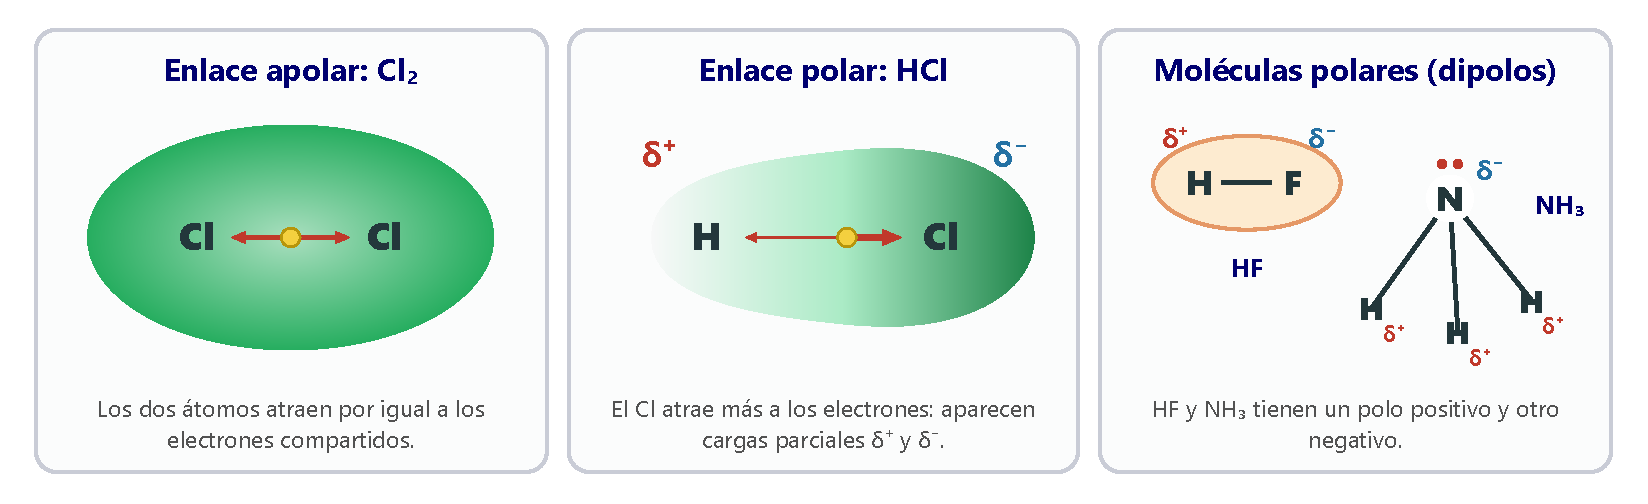
\includegraphics[width=\textwidth]{images/UD3/polaridad}
    \caption{Enlace apolar (\ch{Cl2}), enlace polar (\ch{HCl}) y moléculas polares o dipolos.}
    \label{fig:polaridad}
\end{figure}

\begin{exercise}
    Dibuja una molécula apolar de cloro, \ch{Cl2}, y una molécula polar de bromuro de hidrógeno, \ch{HBr}, indicando las cargas parciales.
    \begin{solu}
        \chemfig{Cl-Cl} (sin cargas parciales: los dos átomos atraen igual a los electrones). \qquad \chemfig{\overset{\delta^+}{\text{H}}-\overset{\delta^-}{\text{Br}}}: el bromo atrae más a los electrones del enlace y queda con la \textcolor{red}{carga parcial negativa}.
    \end{solu}
\end{exercise}

\begin{exercise}
    Corrige las afirmaciones falsas:
    \begin{enumerate}[label=\alph*)]
        \item Un enlace covalente es apolar cuando el centro de las cargas positivas no coincide con el de las negativas.
        \item Un enlace covalente es polar cuando los dos núcleos atraen por igual a los electrones compartidos.
        \item Un enlace covalente es polar cuando un extremo de la molécula tiene carga parcial positiva y el otro negativa.
        \item Un enlace covalente es apolar si uno de los átomos atrae con más fuerza a los electrones.
    \end{enumerate}
    \begin{solu}
        a) \textcolor{red}{Falsa}: es apolar cuando los dos centros \emph{coinciden}. b) \textcolor{red}{Falsa}: en ese caso es \emph{apolar}. c) \textcolor{red}{Verdadera}. d) \textcolor{red}{Falsa}: en ese caso es \emph{polar}.
    \end{solu}
\end{exercise}

%========================================================================================
\section{¿Pueden atraerse los dipolos? Las fuerzas intermoleculares}
%========================================================================================

Las moléculas polares pueden atraerse unas a otras: el extremo positivo de un dipolo atrae al extremo negativo de otro. Estas atracciones entre moléculas se llaman \textbf{fuerzas intermoleculares} y son de dos tipos:
\begin{itemize}
    \item Enlaces o fuerzas de \textbf{hidrógeno}.
    \item Fuerzas de \textbf{Van der Waals}.
\end{itemize}
Son mucho más débiles que los enlaces covalentes. Para distinguirlas, en los dibujos se representan con \textbf{líneas de puntos}.

\subsection{Enlaces o fuerzas de hidrógeno}

\begin{definition}[Enlace de hidrógeno]
    Es la atracción electrostática entre moléculas polares en las que el \textbf{hidrógeno} está unido a un átomo pequeño y con mucha tendencia a captar electrones: \textbf{flúor, oxígeno o nitrógeno}. El hidrógeno de una molécula (\(\delta^+\)) atrae al átomo de F, O o N (\(\delta^-\)) de una molécula vecina.
\end{definition}

\begin{figure}[H]
    \centering
    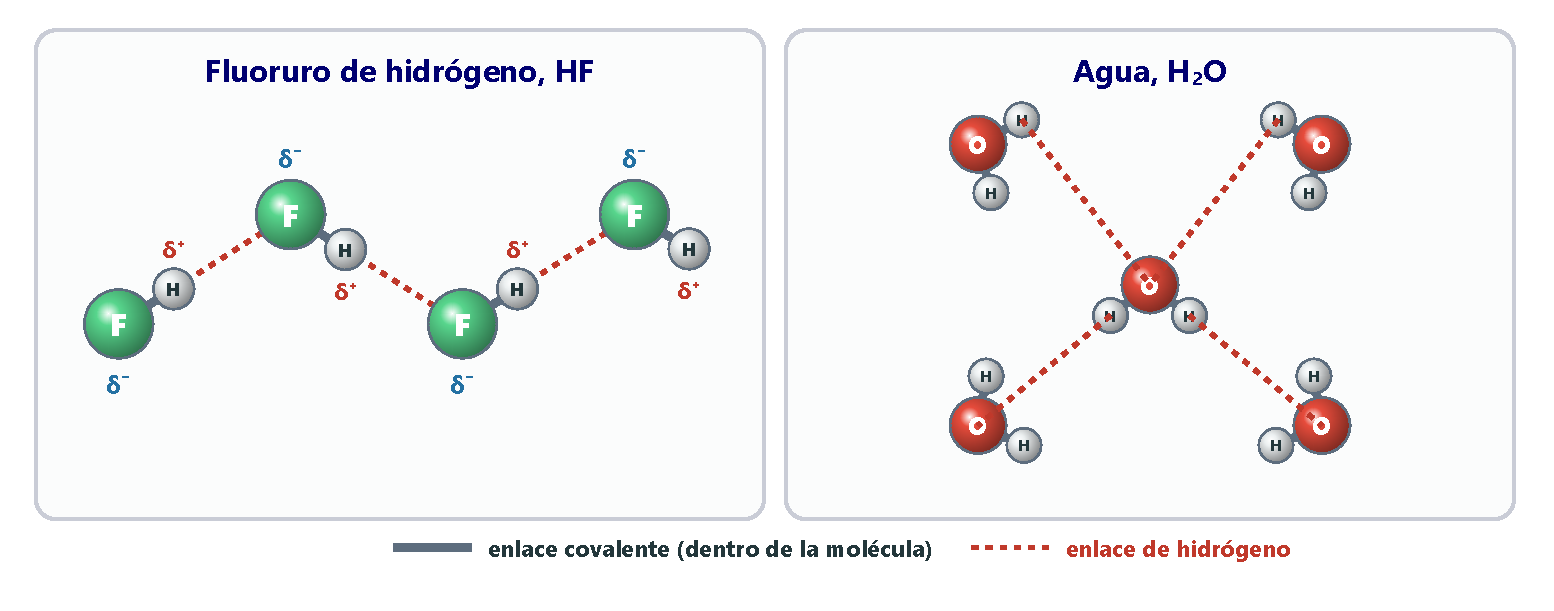
\includegraphics[width=0.85\textwidth]{images/UD3/enlace_hidrogeno}
    \caption{Enlaces de hidrógeno entre moléculas de fluoruro de hidrógeno y entre moléculas de agua.}
    \label{fig:enlace_hidrogeno}
\end{figure}

Estos enlaces mantienen unidas las moléculas de \ch{HF}, \ch{H2O} y \ch{NH3}, de modo que hace falta más energía para separarlas. Por eso sus puntos de fusión y ebullición son \textbf{anormalmente altos} si los comparamos con los de los hidruros de los demás elementos de su grupo (figura~\ref{fig:hidruros_ebullicion}). También hay enlaces de hidrógeno en sustancias como los alcoholes, las proteínas o el ADN.

\begin{figure}[H]
    \centering
    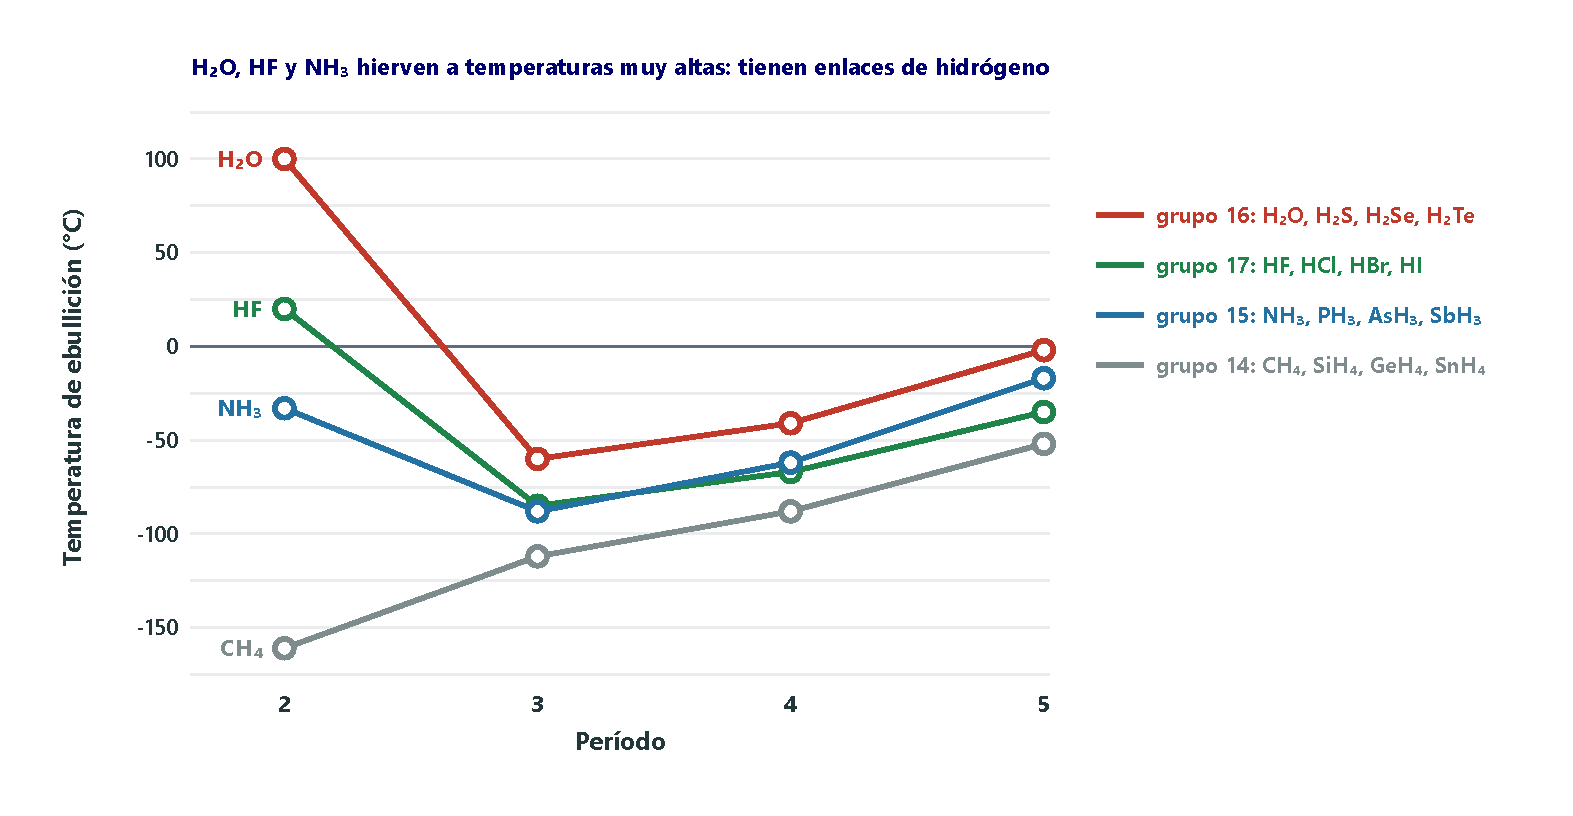
\includegraphics[width=0.9\textwidth]{images/UD3/hidruros_ebullicion}
    \caption{Temperaturas de ebullición de los hidruros de los grupos 14 a 17.}
    \label{fig:hidruros_ebullicion}
\end{figure}

\begin{exercise}
    Las proteínas y los ácidos nucleicos (como el ADN) son macromoléculas formadas sobre todo por carbono, hidrógeno, oxígeno y nitrógeno. Investiga y redacta un breve informe sobre el papel de los enlaces de hidrógeno en estas moléculas.
    \begin{solu}
        Respuesta libre. Por ejemplo: en el ADN, las dos cadenas de la doble hélice se mantienen unidas mediante enlaces de hidrógeno entre las bases nitrogenadas (A--T y G--C); en las proteínas, los enlaces de hidrógeno entre grupos \ch{N-H} y \ch{C=O} dan lugar a estructuras como la hélice \(\upalpha\) y la lámina \(\upbeta\).
    \end{solu}
\end{exercise}

\begin{exercise}
    Dibuja cómo se forman los enlaces de hidrógeno entre moléculas de fluoruro de hidrógeno. Explica por qué el \ch{HF} hierve a una temperatura mucho más alta que el resto de los hidruros del grupo 17.
    \begin{solu}
        \[ \cdots\,\overset{\delta^+}{\text{H}}\!-\!\overset{\delta^-}{\text{F}}\,\cdots\,\overset{\delta^+}{\text{H}}\!-\!\overset{\delta^-}{\text{F}}\,\cdots\,\overset{\delta^+}{\text{H}}\!-\!\overset{\delta^-}{\text{F}}\,\cdots \]
        (las líneas de puntos son los enlaces de hidrógeno; los guiones, los enlaces covalentes). Las moléculas de \ch{HF} no están aisladas: los enlaces de hidrógeno las mantienen unidas y hace falta \textcolor{red}{más energía para separarlas}. En \ch{HCl}, \ch{HBr} y \ch{HI} no hay enlaces de hidrógeno.
    \end{solu}
\end{exercise}

\begin{exercise}
    Dibuja los enlaces de hidrógeno entre moléculas de amoníaco, \ch{NH3}, y justifica por qué su temperatura de ebullición es mayor que la de los hidruros de los demás elementos del grupo 15.
    \begin{solu}
        El nitrógeno (\(\delta^-\)) de una molécula atrae a un hidrógeno (\(\delta^+\)) de la vecina:
        \[ \text{H}_2\overset{\delta^-}{\text{N}}\!-\!\overset{\delta^+}{\text{H}}\,\cdots\,\overset{\delta^-}{\text{N}}\text{H}_2\!-\!\overset{\delta^+}{\text{H}}\,\cdots\,\overset{\delta^-}{\text{N}}\text{H}_3 \]
        Su temperatura de ebullición es mayor porque en \ch{PH3}, \ch{AsH3} y \ch{SbH3} \textcolor{red}{no hay enlaces de hidrógeno}.
    \end{solu}
\end{exercise}

\begin{exercise}
    Analiza la gráfica de la figura~\ref{fig:hidruros_ebullicion} e indica tres hidruros con enlaces de hidrógeno entre sus moléculas y tres en los que no existan o sean muy débiles.
    \begin{solu}
        Con enlaces de hidrógeno: \textcolor{red}{\ch{H2O}, \ch{HF} y \ch{NH3}}, cuyas temperaturas de ebullición son mucho más altas de lo que les correspondería por su tamaño. Sin ellos: por ejemplo, \textcolor{red}{\ch{CH4}, \ch{SiH4} y \ch{GeH4}}.
    \end{solu}
\end{exercise}

\subsection{El agua, una molécula singular}

El oxígeno (\conf{1s^2~2s^2~2p^4}) tiene seis electrones de valencia y le faltan dos; por eso se une a \textbf{dos átomos de hidrógeno}, cada uno con un electrón, mediante dos enlaces covalentes sencillos \ch{O-H}. La molécula es \textbf{angular} y \textbf{polar}: el oxígeno atrae con más fuerza a los electrones y soporta la carga parcial negativa, y los hidrógenos, la positiva. Entre moléculas de agua se forman, por tanto, \textbf{enlaces de hidrógeno}.

\begin{center}
    % --- tabla antigua ---
    % \begin{tblr}{colspec={lcc}, hlines, vlines, row{1}={bg=ocre!85, fg=white, font=\bfseries}, column{1}={bg=ocre!15}, cell{1}{1}={bg=ocre!85, fg=white}}
        % Hidruros del grupo 16 & \(T_\text{f}\) (\unit{\celsius}) & \(T_\text{e}\) (\unit{\celsius}) \\
        % \ch{H2O} & \num{0} & \num{100} \\
        % \ch{H2S} & \num{-82} & \num{-60} \\
        % \ch{H2Se} & \num{-62} & \num{-41} \\
        % \ch{H2Te} & \num{-49} & \num{-1} \\
    % \end{tblr}
    % --- tabla nueva ---
    \begin{tabular}{@{}lcc@{}}
        \toprule
        \textbf{Hidruros del grupo 16} & \textbf{\(T_\text{f}\) (\unit{\celsius})} & \textbf{\(T_\text{e}\) (\unit{\celsius})} \\
        \midrule
        \ch{H2O} & \num{0} & \num{100} \\[3pt]
        \ch{H2S} & \num{-82} & \num{-60} \\[3pt]
        \ch{H2Se} & \num{-62} & \num{-41} \\[3pt]
        \ch{H2Te} & \num{-49} & \num{-1} \\
        \bottomrule
    \end{tabular}
\end{center}

Aunque la molécula de agua es la más pequeña de su grupo, sus puntos de fusión y ebullición son, con diferencia, los más altos. Además:
\begin{itemize}
    \item Es \textbf{líquida} a temperaturas a las que sustancias parecidas ya son gases.
    \item Su densidad aumenta de forma anómala entre \qty{0}{\celsius} y \qty{4}{\celsius}, y el \textbf{hielo es menos denso que el agua líquida}: por eso flota.
\end{itemize}

Las tres cosas se explican por los enlaces de hidrógeno (figura~\ref{fig:agua_estados}):
\begin{itemize}
    \item \textbf{Sólido.} Cada molécula se une a otras formando una red de hexágonos con muchos huecos: el hielo ocupa \textbf{más volumen} que la misma masa de agua líquida.
    \item \textbf{Líquido.} Las moléculas forman grupos que se rompen y se rehacen continuamente; los huecos los ocupan moléculas sueltas, así que el líquido ocupa menos volumen y es más denso.
    \item \textbf{Gas.} Las moléculas están sueltas y muy separadas, sin enlaces de hidrógeno entre ellas.
\end{itemize}

\begin{figure}[H]
    \centering
    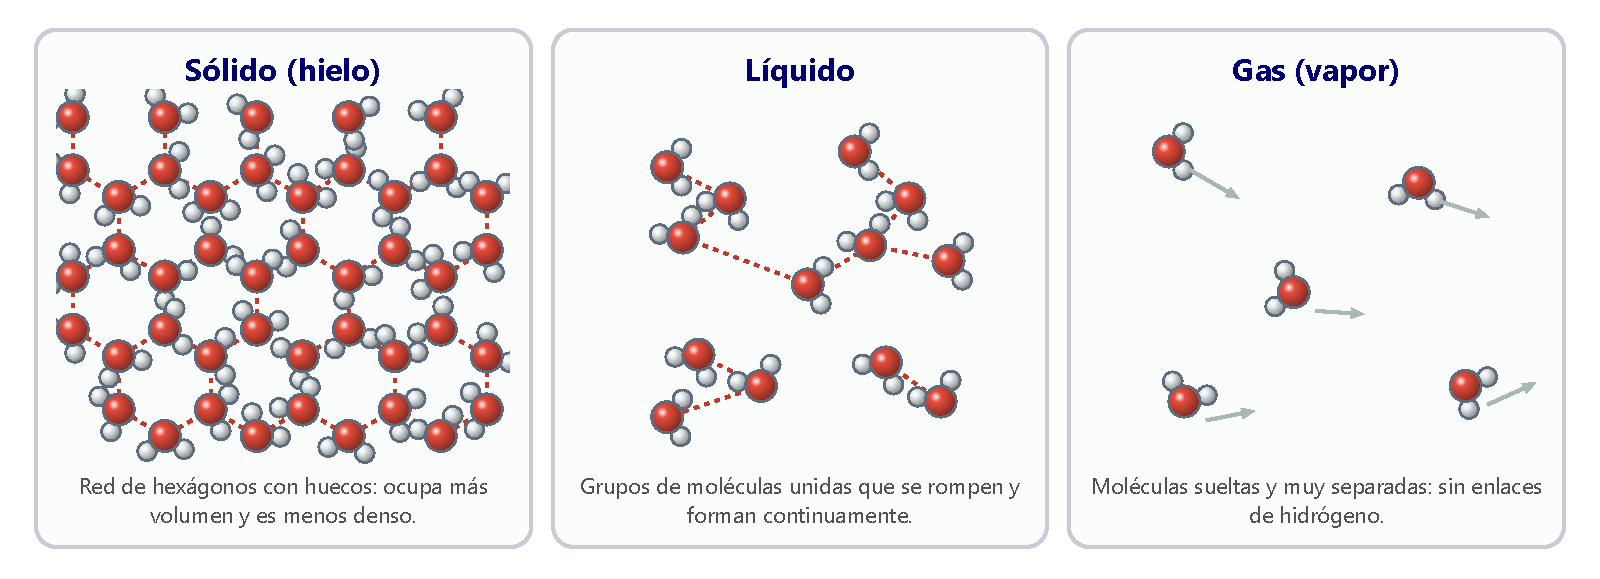
\includegraphics[width=\textwidth]{images/UD3/agua_estados}
    \caption{Enlaces de hidrógeno en el agua sólida, líquida y gaseosa.}
    \label{fig:agua_estados}
\end{figure}

\begin{exercise}
    Escribe el diagrama de Lewis del agua y explica cómo se forman los enlaces covalentes entre el oxígeno y los hidrógenos.
    \begin{solu}
        \chemfig{H-\charge{90=\:,270=\:}{O}-H}. El oxígeno tiene 6 electrones de valencia (\conf{2s^2~2p^4}) y le faltan dos; cada hidrógeno tiene uno y le falta otro. El oxígeno comparte \textcolor{red}{un par de electrones con cada hidrógeno}: se forman \textcolor{red}{dos enlaces covalentes sencillos} \ch{O-H}, y al oxígeno le quedan dos pares sin compartir.
    \end{solu}
\end{exercise}

\begin{exercise}
    ¿Por qué el agua tiene puntos de fusión y ebullición tan distintos de los del \ch{H2S}, el \ch{H2Se} y el \ch{H2Te}?
    \begin{solu}
        Porque entre las moléculas de agua hay \textcolor{red}{enlaces de hidrógeno} (el oxígeno es pequeño y atrae mucho a los electrones), mientras que en los otros hidruros del grupo 16 no los hay. Separar las moléculas de agua cuesta mucha más energía.
    \end{solu}
\end{exercise}

\begin{exercise}
    Observa un cristal de hielo (figura~\ref{fig:agua_estados}).
    \begin{enumerate}[label=\alph*)]
        \item ¿Qué enlaces hay en el cristal?
        \item ¿Qué les ocurre a las moléculas cuando el hielo se funde?
        \item ¿Qué enlaces hay en el agua líquida?
        \item ¿Qué ocurre cuando, finalmente, el agua hierve?
    \end{enumerate}
    \begin{solu}
        a) \textcolor{red}{Enlaces covalentes} \ch{O-H} dentro de cada molécula y \textcolor{red}{enlaces de hidrógeno} entre un H de una molécula y el O de otra. b) Se rompe parte de los enlaces de hidrógeno: las moléculas pierden la estructura de hexágonos y empiezan a moverse unas sobre otras. c) Covalentes dentro de las moléculas y enlaces de hidrógeno que unen grupos de moléculas y se rompen y forman continuamente. d) Se rompen todos los enlaces de hidrógeno: las moléculas quedan \textcolor{red}{sueltas}.
    \end{solu}
\end{exercise}

\subsection{Las fuerzas de Van der Waals}

En una molécula \textbf{apolar} los electrones se mueven continuamente. Si en un instante se acumulan más en un lado que en otro, el centro de las cargas negativas deja de coincidir con el de las positivas y aparece un \textbf{dipolo instantáneo}. Ese dipolo puede deformar la nube de electrones de una molécula vecina y crear en ella un \textbf{dipolo inducido} (figura~\ref{fig:van_der_waals}).

\begin{definition}[Fuerzas de Van der Waals]
    Son fuerzas de atracción electrostática entre \textbf{dipolos instantáneos o inducidos}. Son \textbf{más débiles} que los enlaces de hidrógeno y aparecen entre moléculas apolares (\ch{O2}, \ch{I2}, \ch{CH4}\ldots) e incluso entre átomos aislados (\ch{He}, \ch{Ne}\ldots). Son más intensas cuanto más grande es la molécula, porque tiene más electrones.
\end{definition}

\begin{figure}[H]
    \centering
    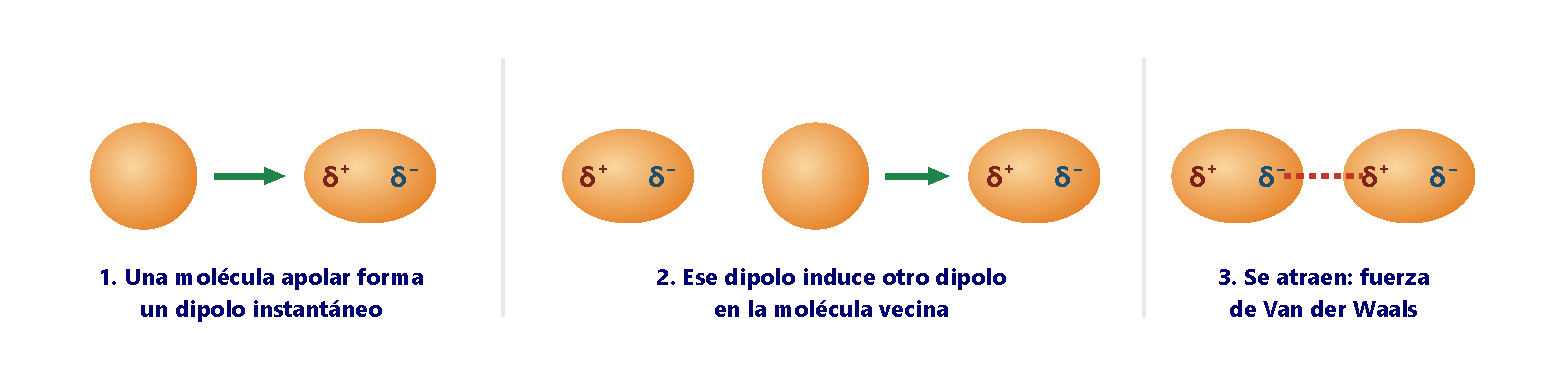
\includegraphics[width=\textwidth]{images/UD3/van_der_waals}
    \caption{Formación de un dipolo instantáneo, de un dipolo inducido y de la fuerza de Van der Waals entre ellos.}
    \label{fig:van_der_waals}
\end{figure}

\begin{remark}
    \textbf{El yodo, un cristal molecular.} El yodo forma cristales de color negro violáceo. Sus puntos de fusión y ebullición son mucho más altos que los del resto de los halógenos, lo que indica que sus moléculas no están aisladas: las moléculas \ch{I2} (dos átomos unidos por un enlace covalente sencillo) se mantienen unidas en una red por \textbf{fuerzas de Van der Waals}. Como estas fuerzas son débiles, el cristal se deshace con facilidad: el yodo \textbf{sublima} a temperatura ambiente. No conduce la electricidad porque no tiene electrones libres.
\end{remark}

\begin{exercise}
    ¿En qué se diferencian un dipolo permanente, uno instantáneo y uno inducido? Dibuja cómo se forma un dipolo instantáneo y cómo induce otro dipolo.
    \begin{solu}
        Un \textcolor{red}{dipolo permanente} (\ch{HCl}, \ch{H2O}\ldots) tiene siempre sus polos. Un \textcolor{red}{dipolo instantáneo} aparece solo durante un instante en una molécula apolar, por el movimiento de sus electrones. Un \textcolor{red}{dipolo inducido} se forma en una molécula apolar por la cercanía de otro dipolo (instantáneo o permanente). Dibujo como el de la figura~\ref{fig:van_der_waals}.
    \end{solu}
\end{exercise}

\begin{exercise}
    Explica las diferencias entre los puntos de fusión y ebullición de los halógenos:
    \begin{center}
        % --- tabla antigua ---
        % \begin{tblr}{colspec={lcc}, hlines, vlines, row{1}={bg=ocre!85, fg=white, font=\bfseries}, column{1}={bg=ocre!15}, cell{1}{1}={bg=ocre!85, fg=white}}
            % Halógeno & \(T_\text{f}\) (\unit{\celsius}) & \(T_\text{e}\) (\unit{\celsius}) \\
            % \ch{F2} & \num{-219.6} & \num{-188.2} \\
            % \ch{Cl2} & \num{-101.0} & \num{-34.7} \\
            % \ch{Br2} & \num{-7.2} & \num{58.8} \\
            % \ch{I2} & \num{113.7} & \num{184.3} \\
        % \end{tblr}
        % --- tabla nueva ---
        \begin{tabular}{@{}lcc@{}}
            \toprule
            \textbf{Halógeno} & \textbf{\(T_\text{f}\) (\unit{\celsius})} & \textbf{\(T_\text{e}\) (\unit{\celsius})} \\
            \midrule
            \ch{F2} & \num{-219.6} & \num{-188.2} \\[3pt]
            \ch{Cl2} & \num{-101.0} & \num{-34.7} \\[3pt]
            \ch{Br2} & \num{-7.2} & \num{58.8} \\[3pt]
            \ch{I2} & \num{113.7} & \num{184.3} \\
            \bottomrule
        \end{tabular}
    \end{center}
    \begin{solu}
        Todos están formados por moléculas apolares unidas por fuerzas de Van der Waals, que son \textcolor{red}{más intensas cuanto más grande es la molécula} (más electrones). Por eso las temperaturas aumentan del flúor al yodo: el flúor y el cloro son gases, el bromo es líquido y el yodo es un \textcolor{red}{sólido} cuyas moléculas forman un cristal molecular.
    \end{solu}
\end{exercise}

\begin{exercise}
    ¿Por qué no conducen la electricidad el yodo ni el diamante, y en cambio el grafito sí?
    \begin{solu}
        En el yodo y en el diamante todos los electrones están fijos en los enlaces: \textcolor{red}{no hay electrones libres}. En el grafito, cada carbono solo forma tres enlaces fuertes y su cuarto electrón \textcolor{red}{puede moverse} a lo largo de las capas.
    \end{solu}
\end{exercise}

\begin{exercise}
    Un elemento del grupo 17 forma, a temperatura ambiente, un sólido en el que las moléculas diatómicas están ordenadas en una red.
    \begin{enumerate}[label=\alph*)]
        \item ¿Puede tratarse del flúor, del cloro o del bromo? Justifícalo.
        \item ¿De qué elemento se trata?
        \item ¿Conduce la corriente eléctrica?
    \end{enumerate}
    \begin{solu}
        a) \textcolor{red}{No}: el flúor y el cloro son gases a temperatura ambiente y el bromo es líquido. b) Del \textcolor{red}{yodo}. c) \textcolor{red}{No}: no tiene electrones libres.
    \end{solu}
\end{exercise}

%========================================================================================
\section{Los compuestos iónicos}
%========================================================================================

Los átomos de muchos \textbf{metales} completan su último nivel \textbf{perdiendo electrones}, mientras que los de muchos \textbf{no metales} lo hacen \textbf{ganándolos}. Cuando se encuentran, el metal cede electrones al no metal: se forman \textbf{cationes} y \textbf{aniones}, que se atraen por tener cargas opuestas.

\subsection{¿Cómo se forma un compuesto iónico? El enlace iónico}

Veamos cómo se forma el cloruro de sodio, la sal común (figura~\ref{fig:formacion_nacl}):

\begin{enumerate}[label=\numberballblue]
    \item \textbf{Formación del ion sodio.} El sodio (\conf{[Ne]~3s^1}) tiene un solo electrón en su último nivel. Al perderlo, se queda con el nivel anterior completo: se forma el catión \ch{Na+}, con 11 protones y 10 electrones.
    \item \textbf{Formación del ion cloruro.} El cloro (\conf{[Ne]~3s^2~3p^5}) tiene siete electrones en su último nivel; al ganar uno lo completa y se convierte en el anión \ch{Cl-}, con 17 protones y 18 electrones.
    \item \textbf{Unión de los iones.} El \ch{Na+} y el \ch{Cl-} tienen cargas opuestas y se atraen por \textbf{fuerzas electrostáticas}: se ha formado un \textbf{enlace iónico}.
    \item \textbf{Formación del cristal.} Cada ion no se une a uno solo, sino que se rodea del mayor número posible de iones de signo contrario: se forma una \textbf{red cristalina iónica}. En el \ch{NaCl}, cada ion está rodeado por \textbf{seis} de signo contrario (figura~\ref{fig:cristal_nacl}).
\end{enumerate}

\begin{figure}[H]
    \centering
    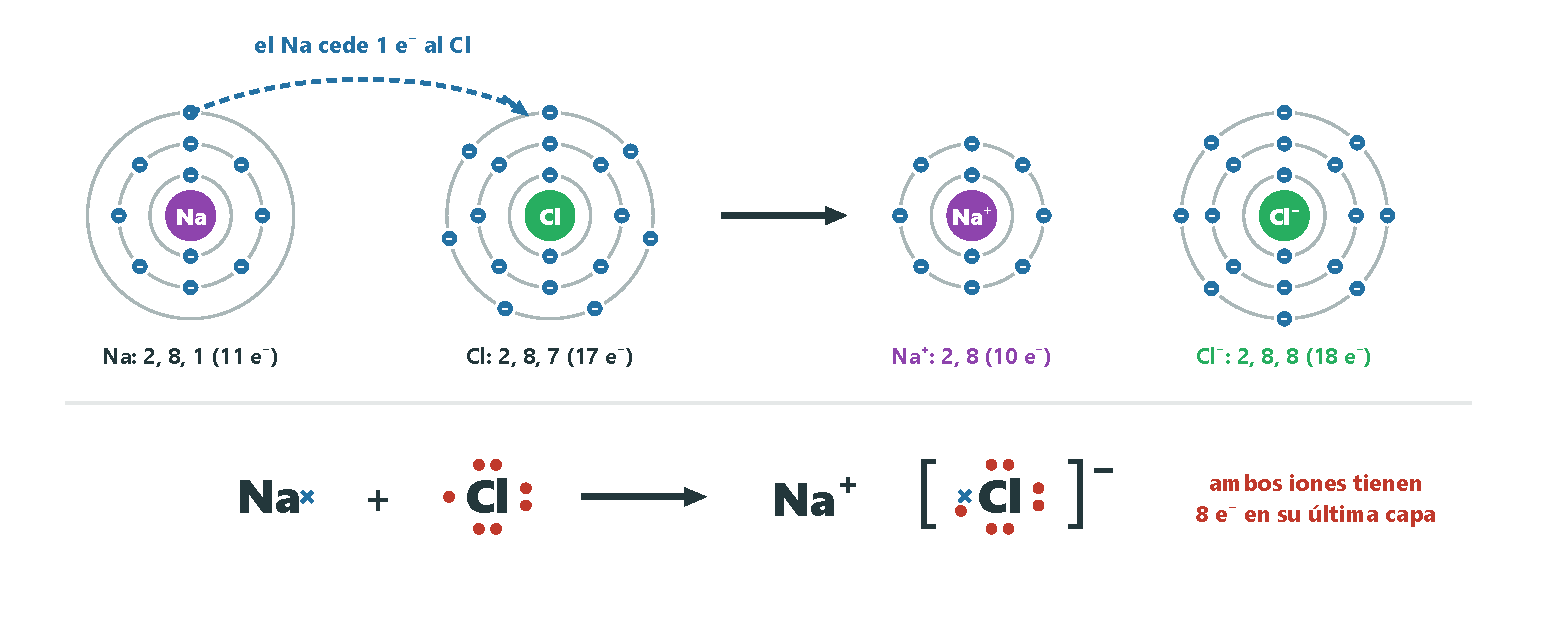
\includegraphics[width=\textwidth]{images/UD3/formacion_nacl}
    \caption{El sodio cede un electrón al cloro: ambos iones consiguen ocho electrones en su último nivel.}
    \label{fig:formacion_nacl}
\end{figure}

\begin{figure}[H]
    \centering
    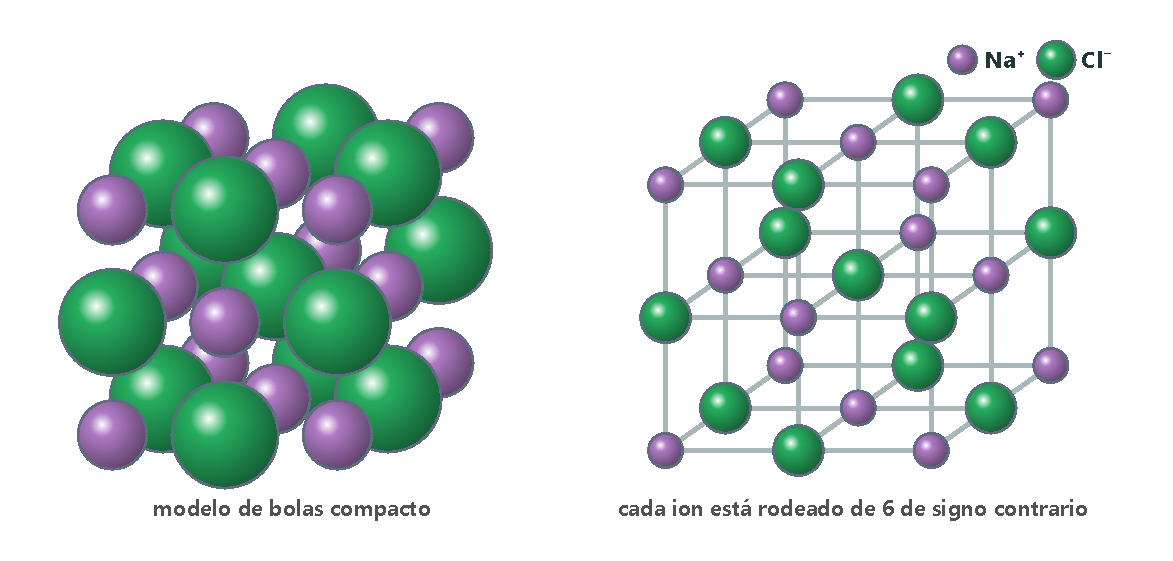
\includegraphics[width=0.75\textwidth]{images/UD3/cristal_nacl}
    \caption{Cristal de cloruro de sodio: modelo de bolas compacto y red cristalina.}
    \label{fig:cristal_nacl}
\end{figure}

\begin{definition}[Enlace iónico]
    Es la unión entre iones de signo contrario mediante fuerzas de atracción electrostática. Se da entre \textbf{metales} (que forman cationes) y \textbf{no metales} (que forman aniones). Los compuestos iónicos son \textbf{cristales}, no moléculas.
\end{definition}

La fórmula de un compuesto iónico solo indica la \textbf{proporción} entre los iones: es una \textbf{fórmula empírica}. \ch{NaCl} significa que hay un ion sodio por cada ion cloruro, y \ch{CaCl2}, que hay dos iones cloruro por cada ion calcio.

\begin{exercise}
    Observa la red de la figura~\ref{fig:cristal_nacl}. ¿Cuántos iones cloruro rodean a cada ion sodio? ¿Y cuántos iones sodio rodean a cada cloruro? ¿En qué proporción están ambos iones?
    \begin{solu}
        Cada \ch{Na+} está rodeado de \textcolor{red}{6} iones \ch{Cl-}, y cada \ch{Cl-}, de \textcolor{red}{6} iones \ch{Na+}. La proporción es \textcolor{red}{1:1}, como indica la fórmula \ch{NaCl}.
    \end{solu}
\end{exercise}

\begin{exercise}
    Explica, paso a paso y con diagramas de Lewis, cómo se forma el fluoruro de litio, \ch{LiF} (\(Z(\ch{Li}) = 3\), \(Z(\ch{F}) = 9\)).
    \begin{solu}
        \textcolor{blue}{1.} El litio (\conf{1s^2~2s^1}) pierde su electrón de valencia y forma \ch{Li+} (configuración del helio). \textcolor{blue}{2.} El flúor (\conf{1s^2~2s^2~2p^5}) gana ese electrón y forma \ch{F-} (configuración del neón). \textcolor{blue}{3.} Los iones se atraen electrostáticamente. \textcolor{blue}{4.} Cada ion se rodea de iones de signo contrario y se forma un cristal iónico.
        \[ \chemfig{\charge{90=\.}{Li}} \;+\; \chemfig{\charge{90=\:,0=\:,270=\:,180=\.}{F}} \;\longrightarrow\; \ch{Li+}\ \text{\ionlewis{\chemfig{\charge{90=\:,0=\:,270=\:,180=\:}{F}}}{-}} \]
    \end{solu}
\end{exercise}

\subsection{¿Qué propiedades tienen los compuestos iónicos?}

El enlace iónico se forma entre metales y no metales. Además del \ch{NaCl}, son compuestos iónicos el fluoruro de litio (\ch{LiF}), el bromuro de potasio (\ch{KBr}), el yoduro de potasio (\ch{KI}), el nitrato de calcio (\ch{Ca(NO3)2}) o el sulfato de bario (\ch{BaSO4}).

\begin{center}
    % --- tabla antigua ---
    % \begin{tblr}{colspec={llcc}, hlines, vlines, row{1}={bg=ocre!85, fg=white, font=\bfseries}, column{1-2}={bg=ocre!15}, cell{1}{1}={c=2}{bg=ocre!85, fg=white}, cell{2}{1}={c=2}{l}, cell{3}{1}={c=2}{l}, cell{4}{1}={c=2}{l}, cell{5}{1}={r=2}{l}, cell{7}{1}={c=2}{l}}
        % Propiedad & & Cloruro de sodio, \ch{NaCl} & Nitrato de calcio, \ch{Ca(NO3)2} \\
        % Aspecto & & cristales incoloros & cristales blancos \\
        % \(T_\text{f}\) (\unit{\celsius}) & & \num{801} & \num{561} \\
        % \(T_\text{e}\) (\unit{\celsius}) & & \num{1465} & se descompone antes \\
        % Conductividad & sólido & muy baja & muy baja \\
        % & fundido & alta & alta \\
        % Solubilidad en agua & & muy alta & alta \\
    % \end{tblr}
    % --- tabla nueva ---
    \begin{tabular}{@{}llcc@{}}
        \toprule
        \multicolumn{2}{c}{\textbf{Propiedad}} & \textbf{Cloruro de sodio, \ch{NaCl}} & \textbf{Nitrato de calcio, \ch{Ca(NO3)2}} \\
        \midrule
        \multicolumn{2}{c}{Aspecto} & cristales incoloros & cristales blancos \\[3pt]
        \multicolumn{2}{c}{\(T_\text{f}\) (\unit{\celsius})} & \num{801} & \num{561} \\[3pt]
        \multicolumn{2}{c}{\(T_\text{e}\) (\unit{\celsius})} & \num{1465} & se descompone antes \\[3pt]
        \multirow{2}{*}{Conductividad} & sólido & muy baja & muy baja \\[3pt]
         & fundido & alta & alta \\[3pt]
        \multicolumn{2}{c}{Solubilidad en agua} & muy alta & alta \\
        \bottomrule
    \end{tabular}
\end{center}

\begin{center}
    % --- tabla antigua ---
    % \begin{tblr}{colspec={X[3,l]X[5,l]}, hlines, vlines, row{1}={bg=ocre!85, fg=white, font=\bfseries, halign=c}}
        % Propiedad & Justificación \\
        % Son \textbf{sólidos cristalinos} a temperatura ambiente. & La atracción entre iones es muy intensa y se extiende en todas las direcciones: cada ion queda rodeado de iones de carga opuesta formando una red. \\
        % Tienen puntos de fusión y ebullición \textbf{elevados}. & Para que los iones abandonen sus posiciones en la red hay que vencer fuerzas muy intensas, lo que requiere mucha energía. \\
        % Son \textbf{duros}. & Para rayarlos hay que romper las fuertes uniones entre los iones. \\
        % Son \textbf{frágiles}. & Al golpearlos, una capa de iones se desplaza y quedan enfrentados iones del mismo signo, que se repelen: el cristal se rompe (figura~\ref{fig:golpe_ionico_metal}). \\
        % Muchos son \textbf{solubles en agua}. & Los dipolos del agua rodean a los iones y los separan de la red; se orientan de forma distinta según rodeen a un catión o a un anión (figura~\ref{fig:disolucion_ionico}). \\
        % \textbf{No conducen} la electricidad en estado sólido. & Los electrones están fijos en los iones y los iones no pueden moverse dentro del cristal. \\
        % \textbf{Conducen} la electricidad fundidos o disueltos. & Al fundirse o disolverse, los iones quedan libres y pueden transportar la corriente. \\
    % \end{tblr}
    % --- tabla nueva ---
    \begin{tabular}{@{}L{0.34\linewidth} L{0.57\linewidth}@{}}
        \toprule
        \textbf{Propiedad} & \textbf{Justificación} \\
        \midrule
        Son \textbf{sólidos cristalinos} a temperatura ambiente. & La atracción entre iones es muy intensa y se extiende en todas las direcciones: cada ion queda rodeado de iones de carga opuesta formando una red. \\[3pt]
        Tienen puntos de fusión y ebullición \textbf{elevados}. & Para que los iones abandonen sus posiciones en la red hay que vencer fuerzas muy intensas, lo que requiere mucha energía. \\[3pt]
        Son \textbf{duros}. & Para rayarlos hay que romper las fuertes uniones entre los iones. \\[3pt]
        Son \textbf{frágiles}. & Al golpearlos, una capa de iones se desplaza y quedan enfrentados iones del mismo signo, que se repelen: el cristal se rompe (figura~\ref{fig:golpe_ionico_metal}). \\[3pt]
        Muchos son \textbf{solubles en agua}. & Los dipolos del agua rodean a los iones y los separan de la red; se orientan de forma distinta según rodeen a un catión o a un anión (figura~\ref{fig:disolucion_ionico}). \\[3pt]
        \textbf{No conducen} la electricidad en estado sólido. & Los electrones están fijos en los iones y los iones no pueden moverse dentro del cristal. \\[3pt]
        \textbf{Conducen} la electricidad fundidos o disueltos. & Al fundirse o disolverse, los iones quedan libres y pueden transportar la corriente. \\
        \bottomrule
    \end{tabular}
\end{center}

\begin{figure}[H]
    \centering
    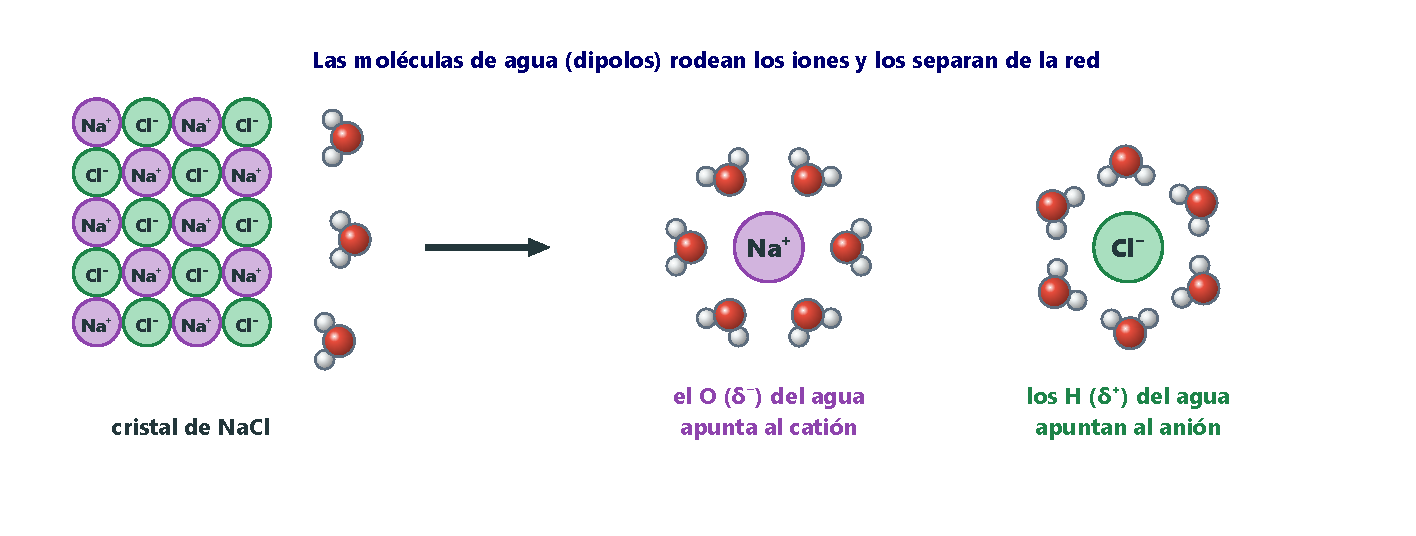
\includegraphics[width=0.85\textwidth]{images/UD3/disolucion_ionico}
    \caption{Disolución de un compuesto iónico en agua.}
    \label{fig:disolucion_ionico}
\end{figure}

\begin{exercise}
    Explica por qué el hecho de que la molécula de agua sea un dipolo facilita la disolución de los compuestos iónicos. Haz un dibujo del proceso.
    \begin{solu}
        Las moléculas de agua, que son dipolos, \textcolor{red}{rodean a los iones} del cristal y los separan de la red: orientan su extremo negativo (el oxígeno) hacia los cationes y su extremo positivo (los hidrógenos) hacia los aniones. Dibujo como el de la figura~\ref{fig:disolucion_ionico}.
    \end{solu}
\end{exercise}

\begin{exercise}
    Tienes dos frascos sin etiqueta con dos sólidos cristalinos de aspecto muy parecido. Uno es un compuesto iónico y el otro un compuesto covalente reticular. Si solo dispones de agua, ¿qué prueba harías para distinguirlos?
    \begin{solu}
        Intentaría disolver un poco de cada uno en agua: el que se disuelva será el \textcolor{red}{compuesto iónico} y el que no, el \textcolor{red}{covalente reticular}. (Además, la disolución del iónico conduciría la electricidad.)
    \end{solu}
\end{exercise}

\begin{exercise}
    Clasifica estos compuestos en iónicos o covalentes: \ch{CO2}, \ch{NaF}, \ch{H2S}, \ch{SiO2}, \ch{CaO}, \ch{NH3}, \ch{KBr}, \ch{HCl}.
    \begin{solu}
        \textcolor{blue}{Metal + no metal \(\to\) iónico; no metal + no metal \(\to\) covalente.} Iónicos: \textcolor{red}{\ch{NaF}, \ch{CaO}, \ch{KBr}}. Covalentes: \textcolor{red}{\ch{CO2}, \ch{H2S}, \ch{SiO2}, \ch{NH3}, \ch{HCl}}.
    \end{solu}
\end{exercise}

\begin{exercise}
    Indica si cada propiedad la presentan los compuestos covalentes cristalinos, los iónicos o ambos:
    \begin{enumerate}[label=\alph*)]
        \item Son sólidos cristalinos.
        \item Son muy duros.
        \item Tienen puntos de fusión y ebullición elevados.
        \item No conducen la electricidad en estado sólido.
        \item Se disuelven en agua.
        \item No se disuelven en agua.
        \item Conducen la electricidad fundidos o disueltos.
        \item Están formados por cationes y aniones.
    \end{enumerate}
    \begin{solu}
        a), b), c) y d): \textcolor{red}{ambos}. e) \textcolor{red}{Iónicos}. f) \textcolor{red}{Covalentes}. g) \textcolor{red}{Iónicos}. h) \textcolor{red}{Iónicos}.
    \end{solu}
\end{exercise}

\begin{exercise}
    La tabla recoge algunas propiedades de cuatro sustancias:
    \begin{center}
        % --- tabla antigua ---
        % \begin{tblr}{colspec={ccccc}, hlines, vlines, row{1-2}={bg=ocre!85, fg=white, font=\bfseries}, cell{1}{1}={r=2}{}, cell{1}{2}={r=2}{}, cell{1}{3}={c=2}{}, cell{1}{5}={r=2}{}}
            % Sustancia & \(T_\text{f}\) (\unit{\celsius}) & Conductividad & & ¿Soluble en agua? \\
            % & & sólido & disuelto & \\
            % A & \num{114} & no & no & no \\
            % B & \num{770} & no & sí & sí \\
            % C & \num{1710} & no & no & no \\
            % D & \num{690} & no & sí & sí \\
        % \end{tblr}
        % --- tabla nueva ---
        \begin{tabular}{@{}ccccc@{}}
            \toprule
            \multirow{2}{*}{\textbf{Sustancia}} & \multirow{2}{*}{\textbf{\(T_\text{f}\) (\unit{\celsius})}} & \multicolumn{2}{c}{\textbf{Conductividad}} & \multirow{2}{*}{\textbf{¿Soluble en agua?}} \\[3pt]
             &  & \textbf{sólido} & \textbf{disuelto} &  \\[3pt]
            A & \num{114} & no & no & no \\[3pt]
            B & \num{770} & no & sí & sí \\[3pt]
            C & \num{1710} & no & no & no \\[3pt]
            D & \num{690} & no & sí & sí \\
            \bottomrule
        \end{tabular}
    \end{center}
    \begin{enumerate}[label=\alph*)]
        \item ¿Cuáles son compuestos iónicos?
        \item ¿Cuál es un compuesto covalente molecular?
        \item ¿Cuál tiene un punto de fusión muy alto comparado con las demás? ¿Por qué no puede ser iónico?
    \end{enumerate}
    \begin{solu}
        a) \textcolor{red}{B y D}: se disuelven en agua y la disolución conduce. b) \textcolor{red}{A}: punto de fusión bajo, no conduce y no es soluble. c) \textcolor{red}{C}; no es iónico porque \textcolor{red}{no se disuelve} en agua: es un compuesto covalente reticular.
    \end{solu}
\end{exercise}

\begin{exercise}
    En un laboratorio se han obtenido cuatro sustancias sólidas, ninguna de las cuales conduce la electricidad en estado sólido:
    \begin{center}
        % --- tabla antigua ---
        % \begin{tblr}{colspec={X[c]X[c]X[c]X[c]}, hlines, vlines, row{1}={bg=ocre!85, fg=white, font=\bfseries}}
            % Sustancia A & Sustancia B & Sustancia C & Sustancia D \\
            % Formada por átomos de un solo elemento & Formada por dos elementos diferentes & Formada por dos elementos diferentes & Formada por dos elementos diferentes \\
            % Puntos de fusión y ebullición bajos & Puntos de fusión y ebullición elevados & Puntos de fusión y ebullición bajos & Puntos de fusión y ebullición elevados \\
            % Se disuelve en tetracloruro de carbono & No se disuelve en agua & No se disuelve en agua & Se disuelve en agua \\
        % \end{tblr}
        % --- tabla nueva ---
        \begin{tabular}{@{}C{0.21\linewidth} C{0.21\linewidth} C{0.21\linewidth} C{0.21\linewidth}@{}}
            \toprule
            \textbf{Sustancia A} & \textbf{Sustancia B} & \textbf{Sustancia C} & \textbf{Sustancia D} \\
            \midrule
            Formada por átomos de un solo elemento & Formada por dos elementos diferentes & Formada por dos elementos diferentes & Formada por dos elementos diferentes \\[3pt]
            Puntos de fusión y ebullición bajos & Puntos de fusión y ebullición elevados & Puntos de fusión y ebullición bajos & Puntos de fusión y ebullición elevados \\[3pt]
            Se disuelve en tetracloruro de carbono & No se disuelve en agua & No se disuelve en agua & Se disuelve en agua \\
            \bottomrule
        \end{tabular}
    \end{center}
    \begin{enumerate}[label=\alph*)]
        \item ¿Qué tipo de enlace propondrías para cada una?
        \item Si solo pudieras pedir \emph{una} prueba más para cada sustancia (conductividad fundida o disuelta, dureza, solubilidad en tetracloruro de carbono o fragilidad), ¿cuál elegirías para confirmar tu hipótesis?
    \end{enumerate}
    \begin{solu}
        a) A: \textcolor{red}{elemento que forma un cristal covalente molecular} (como el yodo). B: \textcolor{red}{compuesto covalente reticular}. C: \textcolor{red}{compuesto covalente molecular}. D: \textcolor{red}{compuesto iónico}.
        b) A: fragilidad (los cristales moleculares se deshacen con facilidad). B: dureza (los reticulares son muy duros). C: solubilidad en tetracloruro de carbono (los moleculares se disuelven en disolventes apolares). D: conductividad fundida o disuelta (los iónicos conducen en esos estados).
    \end{solu}
\end{exercise}

\begin{exercise}
    Explica, siguiendo los cuatro pasos de esta sección, cómo se forma un cristal de bromuro de potasio, \ch{KBr} (\(Z(\ch{K}) = 19\), \(Z(\ch{Br}) = 35\)).
    \begin{solu}
        \textcolor{blue}{1. Ion potasio:} el K (\conf{[Ar]~4s^1}) pierde su único electrón de valencia y forma \ch{K+}. \textcolor{blue}{2. Ion bromuro:} el Br (\conf{[Ar]~4s^2~3d^{10}~4p^5}) gana ese electrón y forma \ch{Br-}. \textcolor{blue}{3. Unión:} los iones de signo contrario se atraen por fuerzas electrostáticas (enlace iónico). \textcolor{blue}{4. Cristal:} cada ion se rodea del máximo número posible de iones de signo contrario y se forma una \textcolor{red}{red cristalina iónica} con proporción 1:1.
    \end{solu}
\end{exercise}

%========================================================================================
\section{El enlace metálico}
%========================================================================================

Los metales tienen propiedades muy diferentes de las del resto de los elementos porque sus átomos se unen mediante un enlace específico. Sus átomos suelen tener \textbf{uno, dos o tres electrones} en el último nivel, débilmente atraídos por el núcleo, por lo que pueden desplazarse o cederse con facilidad. El carácter metálico aumenta hacia la izquierda y hacia abajo en la tabla periódica.

Según la \textbf{teoría de los electrones libres}, cuando los átomos de un metal se aproximan todo lo posible, sus niveles exteriores se solapan y sus electrones de valencia dejan de pertenecer a un átomo concreto: se convierten en \textbf{electrones libres deslocalizados}.

\begin{definition}[Enlace metálico]
    Un \textbf{cristal metálico} está formado por \textbf{cationes} fijos y perfectamente ordenados, sumergidos en un «mar» o «gas» de \textbf{electrones libres} que se mueven por todo el cristal y mantienen unidos a los cationes.
\end{definition}

\begin{figure}[H]
    \centering
    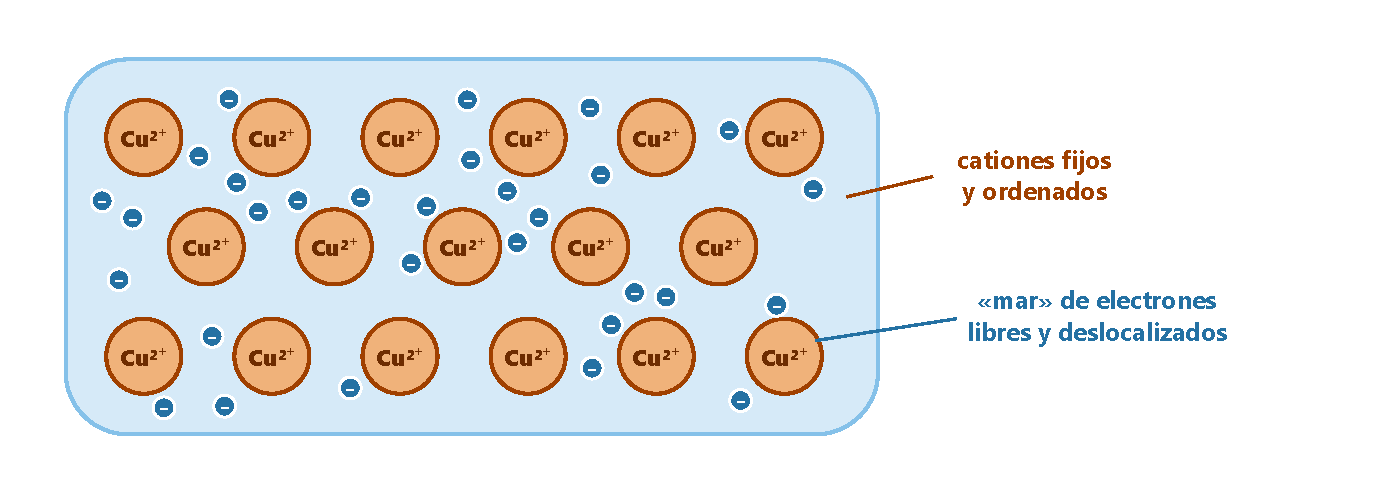
\includegraphics[width=0.8\textwidth]{images/UD3/enlace_metalico}
    \caption{Modelo del mar de electrones en un cristal de cobre.}
    \label{fig:enlace_metalico}
\end{figure}

Los átomos de los metales están muy \textbf{empaquetados}, por eso la densidad de los metales suele ser elevada. Los menos densos son los alcalinos (el litio flota en el agua) y el más denso es el osmio, con \qty{22.6}{\gram\per\cubic\centi\metre}.

\subsection{¿Cómo explica la teoría de los electrones libres las propiedades de los metales?}

\begin{itemize}
    \item \textbf{Duros, dúctiles y maleables.} Sus átomos están muy juntos, por lo que son difíciles de rayar. Sin embargo, una fuerza externa puede hacer que una capa de cationes se deslice sobre otra sin que el cristal se rompa, porque el mar de electrones sigue uniéndolos. Por eso los metales se pueden estirar en hilos (\textbf{ductilidad}) y extender en láminas (\textbf{maleabilidad}).
    \item \textbf{Buenos conductores de la electricidad.} Los electrones libres se mueven con facilidad hacia el polo positivo cuando se aplica una diferencia de potencial. La conductividad disminuye cuando el metal se funde.
    \item \textbf{Buenos conductores del calor.} Si se calienta una zona del metal, sus cationes vibran más y transmiten esa energía rápidamente a los vecinos (y también la transportan los electrones libres).
    \item \textbf{Puntos de fusión y ebullición elevados}, en general, porque hay que separar los átomos de una red muy compacta. Varían mucho: el mercurio es líquido a temperatura ambiente y el wolframio funde a \qty{3380}{\celsius}.
    \item \textbf{Brillo metálico}: reflejan casi toda la luz que reciben.
\end{itemize}

\begin{figure}[H]
    \centering
    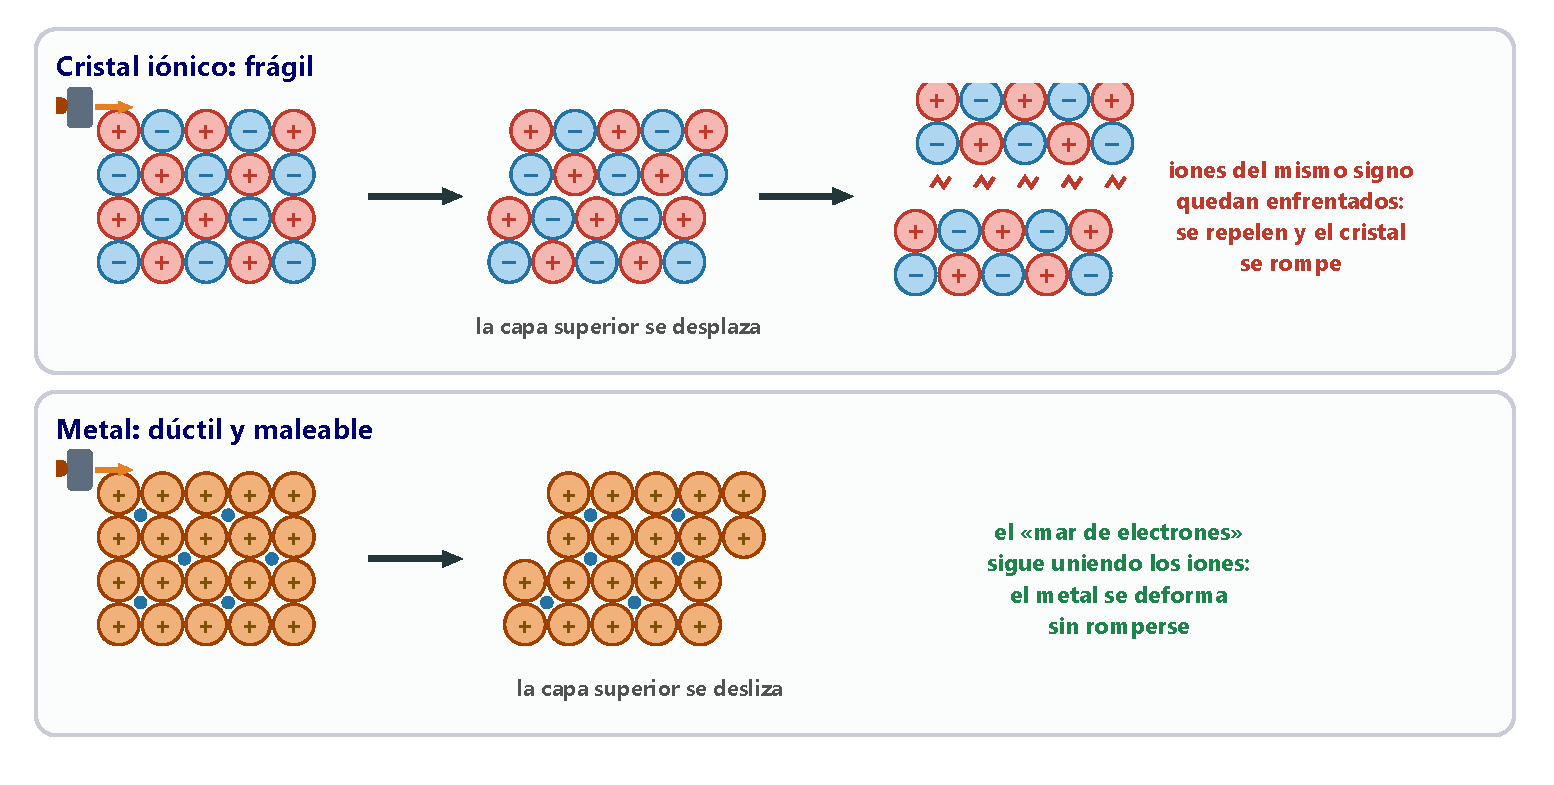
\includegraphics[width=\textwidth]{images/UD3/golpe_ionico_metal}
    \caption{Al golpear un cristal iónico, se enfrentan iones del mismo signo y se rompe; un metal se deforma sin romperse.}
    \label{fig:golpe_ionico_metal}
\end{figure}

\begin{example}
    \textbf{Ejercicio resuelto.} Estas dos gráficas muestran cómo varía la conductividad eléctrica de dos sólidos al calentarlos. ¿Cuál corresponde a un cristal iónico y cuál a uno metálico?

    \begin{center}
        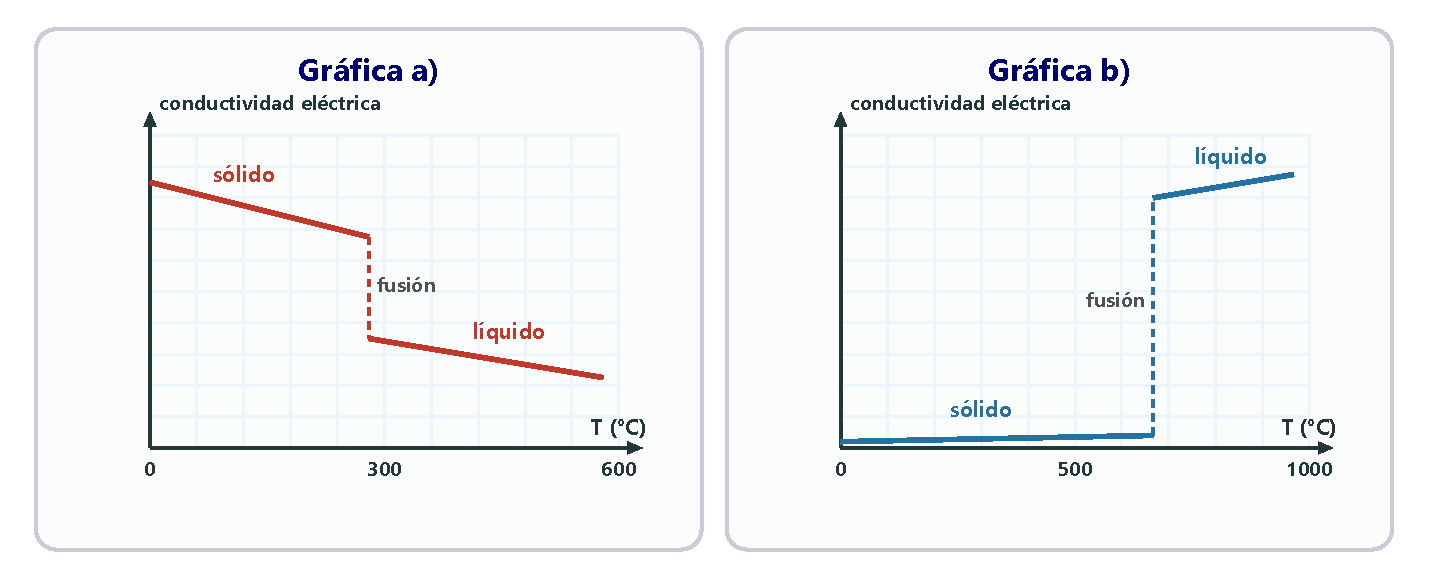
\includegraphics[width=0.8\textwidth]{images/UD3/conductividad_graficas}
    \end{center}

    \textcolor{blue}{Gráfica a):} la conductividad del sólido es muy alta, pero baja bruscamente al fundirse y es pequeña en el líquido. Es un \textcolor{red}{cristal metálico}: buen conductor en estado sólido, pero no tanto fundido.

    \textcolor{blue}{Gráfica b):} el sólido casi no conduce, pero la conductividad sube de golpe al fundirse. Es un \textcolor{red}{cristal iónico}: en el sólido no hay cargas que puedan moverse y, al fundirse, los iones quedan libres.
\end{example}

\begin{exercise}
    ¿Por qué los metales suelen tener densidades elevadas?
    \begin{solu}
        Porque sus átomos están muy \textcolor{red}{empaquetados}: en un volumen dado hay muchos átomos y, por tanto, mucha masa.
    \end{solu}
\end{exercise}

\begin{exercise}
    Busca la densidad de estos metales y ordénalos de menor a mayor: oro, potasio, aluminio, litio, plomo, sodio, hierro, platino.
    \begin{solu}
        \textcolor{blue}{Densidades aproximadas en \unit{\gram\per\cubic\centi\metre}:} Li \num{0.53}, K \num{0.86}, Na \num{0.97}, Al \num{2.70}, Fe \num{7.87}, Pb \num{11.3}, Au \num{19.3}, Pt \num{21.4}.
        \textcolor{red}{Li \(<\) K \(<\) Na \(<\) Al \(<\) Fe \(<\) Pb \(<\) Au \(<\) Pt}.
    \end{solu}
\end{exercise}

\begin{exercise}
    Explica con la teoría de los electrones libres por qué los metales conducen la electricidad.
    \begin{solu}
        Los electrones del enlace metálico están \textcolor{red}{libres y deslocalizados}: no pertenecen a ningún átomo y pueden moverse con gran facilidad por el cristal. Al aplicar una diferencia de potencial, se desplazan hacia el polo positivo: hay corriente eléctrica.
    \end{solu}
\end{exercise}

\begin{exercise}
    Compara lo que ocurre al golpear un sólido iónico y un metal. ¿Por qué el primero es frágil y el segundo dúctil y maleable?
    \begin{solu}
        En el sólido iónico, el golpe desplaza una capa de iones y quedan \textcolor{red}{enfrentados iones del mismo signo}, que se repelen: el cristal se rompe a lo largo de ese plano. En el metal, una capa de cationes se desliza sobre otra pero el \textcolor{red}{mar de electrones sigue uniéndolos}: el metal se deforma sin romperse (figura~\ref{fig:golpe_ionico_metal}).
    \end{solu}
\end{exercise}

\begin{exercise}
    Dadas las especies químicas \ch{Na+}, \ch{Br-}, \ch{He}, \ch{Cu}, \ch{N2}, \ch{CO2}, \ch{MgCl2}, elige:
    \begin{enumerate}[label=\alph*)]
        \item dos átomos;
        \item dos iones;
        \item dos elementos;
        \item dos moléculas;
        \item dos compuestos;
        \item un metal y un no metal.
    \end{enumerate}
    \begin{solu}
        a) \ch{He} y \ch{Cu}. b) \ch{Na+} y \ch{Br-}. c) Por ejemplo, \ch{Cu} y \ch{N2}. d) \ch{N2} y \ch{CO2}. e) \ch{CO2} y \ch{MgCl2}. f) \ch{Cu} (metal) y \ch{He} o \ch{N2} (no metales).
    \end{solu}
\end{exercise}

\begin{exercise}
    Indica qué afirmaciones son verdaderas y corrige las falsas:
    \begin{enumerate}[label=\alph*)]
        \item En el enlace metálico los electrones no pertenecen a ningún átomo concreto.
        \item Los metales se rayan con facilidad.
        \item Los metales funden a temperaturas bajas porque sus átomos se separan fácilmente.
        \item Los metales no conducen la electricidad porque no tienen electrones libres.
        \item Los metales tienen brillo.
        \item Los metales son buenos conductores del calor.
    \end{enumerate}
    \begin{solu}
        a) \textcolor{red}{Verdadera}. b) \textcolor{red}{Falsa}: sus átomos están muy juntos y son difíciles de rayar. c) \textcolor{red}{Falsa}: en general hace falta mucha energía para separar los átomos de la red, por lo que sus puntos de fusión son elevados. d) \textcolor{red}{Falsa}: gracias a sus electrones libres son muy buenos conductores. e) \textcolor{red}{Verdadera}. f) \textcolor{red}{Verdadera}.
    \end{solu}
\end{exercise}

\begin{exercise}
    Indica qué tipo de sustancia forma cada elemento (átomos aislados, moléculas covalentes, cristal covalente atómico, cristal covalente molecular o cristal metálico): \ch{Ne}, \ch{Al}, \ch{O2}, \ch{I2}, carbono (grafito), \ch{Ag}, carbono (diamante), \ch{Kr}, \ch{Pt}. ¿Cuáles conducen la electricidad?
    \begin{solu}
        Átomos aislados: \ch{Ne}, \ch{Kr}. Moléculas covalentes: \ch{O2}. Cristal covalente molecular: \ch{I2}. Cristales covalentes atómicos: grafito y diamante. Cristales metálicos: \ch{Al}, \ch{Ag}, \ch{Pt}.
        Conducen la electricidad: \textcolor{red}{\ch{Al}, \ch{Ag}, \ch{Pt} y el grafito}.
    \end{solu}
\end{exercise}

%========================================================================================
\section{Cantidad de sustancia. El mol y la masa molar}
%========================================================================================

En la tabla periódica aparece la masa atómica relativa de cada elemento. A partir de ellas podemos calcular la masa de las moléculas y de los compuestos.

\subsection{La masa molecular relativa}

\begin{definition}[Masa molecular relativa, \(M_r\)]
    La \textbf{masa molecular relativa} (o simplemente masa molecular) de un elemento o compuesto es la \textbf{suma de las masas atómicas relativas} de todos los átomos que aparecen en su fórmula. No tiene unidades.
\end{definition}

Se calcula igual sea cual sea la forma en que se presenta la sustancia:

\begin{center}
    % --- tabla antigua ---
    % \begin{tblr}{colspec={X[3,l]X[4,l]}, hlines, vlines, row{1}={bg=ocre!85, fg=white, font=\bfseries, halign=c}}
        % Tipo de sustancia & Ejemplo \\
        % Elemento formado por átomos aislados & \(M_r(\ch{Ne}) = A_r(\ch{Ne}) = \num{20.18}\) \\
        % Elemento formado por moléculas & \(M_r(\ch{O2}) = 2 \cdot 16 = 32\); \quad \(M_r(\ch{N2}) = 2 \cdot 14 = 28\) \\
        % Elemento en forma de cristal (covalente o metálico) & \(M_r(\ch{C}) = 12\); \quad \(M_r(\ch{Fe}) = 56\) \\
        % Compuesto iónico & \(M_r(\ch{NaCl}) = 23 + \num{35.5} = \num{58.5}\) (la fórmula solo indica la proporción de iones) \\
        % Compuesto covalente reticular & \(M_r(\ch{SiO2}) = 28 + 2 \cdot 16 = 60\) \\
        % Compuesto covalente molecular & \(M_r(\ch{H2O}) = 2 \cdot 1 + 16 = 18\); \quad \(M_r(\ch{HCl}) = 1 + \num{35.5} = \num{36.5}\) \\
    % \end{tblr}
    % --- tabla nueva ---
    \begin{tabular}{@{}L{0.39\linewidth} L{0.52\linewidth}@{}}
        \toprule
        \textbf{Tipo de sustancia} & \textbf{Ejemplo} \\
        \midrule
        Elemento formado por átomos aislados & \(M_r(\ch{Ne}) = A_r(\ch{Ne}) = \num{20.18}\) \\[3pt]
        Elemento formado por moléculas & \(M_r(\ch{O2}) = 2 \cdot 16 = 32\); \quad \(M_r(\ch{N2}) = 2 \cdot 14 = 28\) \\[3pt]
        Elemento en forma de cristal (covalente o metálico) & \(M_r(\ch{C}) = 12\); \quad \(M_r(\ch{Fe}) = 56\) \\[3pt]
        Compuesto iónico & \(M_r(\ch{NaCl}) = 23 + \num{35.5} = \num{58.5}\) (la fórmula solo indica la proporción de iones) \\[3pt]
        Compuesto covalente reticular & \(M_r(\ch{SiO2}) = 28 + 2 \cdot 16 = 60\) \\[3pt]
        Compuesto covalente molecular & \(M_r(\ch{H2O}) = 2 \cdot 1 + 16 = 18\); \quad \(M_r(\ch{HCl}) = 1 + \num{35.5} = \num{36.5}\) \\
        \bottomrule
    \end{tabular}
\end{center}

\begin{remark}
    \textbf{Masas atómicas que usaremos en esta sección:} H = 1; C = 12; N = 14; O = 16; F = 19; Na = 23; Mg = 24; Al = 27; Si = 28; S = 32; Cl = \num{35.5}; K = 39; Ca = 40; Fe = 56; Cu = \num{63.5}; Br = 80; Ag = 108; I = 127; Au = 197.
\end{remark}

\begin{exercise}
    Calcula la masa molecular relativa de:
    \begin{enumerate}[label=\alph*)]
        \item Dos elementos formados por átomos aislados: neón (\(A_r = \num{20.18}\)) y criptón (\(A_r = \num{83.80}\)).
        \item Tres elementos que forman cristales metálicos: potasio, plata y oro.
    \end{enumerate}
    \begin{solu}
        \textcolor{blue}{En los átomos aislados y en los cristales la masa molecular coincide con la masa atómica:}
        a) \(M_r(\ch{Ne}) = \textcolor{red}{\num{20.18}}\); \(M_r(\ch{Kr}) = \textcolor{red}{\num{83.80}}\). b) \(M_r(\ch{K}) = \textcolor{red}{39}\); \(M_r(\ch{Ag}) = \textcolor{red}{108}\); \(M_r(\ch{Au}) = \textcolor{red}{197}\).
    \end{solu}
\end{exercise}

\begin{exercise}
    Calcula la masa molecular relativa de estos elementos moleculares: oxígeno, \ch{O2}; cloro, \ch{Cl2}; yodo, \ch{I2}; nitrógeno, \ch{N2}.
    \begin{solu}
        \(M_r(\ch{O2}) = 2 \cdot 16 = \textcolor{red}{32}\); \(M_r(\ch{Cl2}) = 2 \cdot \num{35.5} = \textcolor{red}{71}\); \(M_r(\ch{I2}) = 2 \cdot 127 = \textcolor{red}{254}\); \(M_r(\ch{N2}) = 2 \cdot 14 = \textcolor{red}{28}\).
    \end{solu}
\end{exercise}

\begin{exercise}
    Calcula la masa molecular relativa de estos compuestos moleculares: dióxido de carbono, \ch{CO2}; sulfuro de hidrógeno, \ch{H2S}; trióxido de azufre, \ch{SO3}.
    \begin{solu}
        \(M_r(\ch{CO2}) = 12 + 2 \cdot 16 = \textcolor{red}{44}\); \(M_r(\ch{H2S}) = 2 \cdot 1 + 32 = \textcolor{red}{34}\); \(M_r(\ch{SO3}) = 32 + 3 \cdot 16 = \textcolor{red}{80}\).
    \end{solu}
\end{exercise}

\begin{exercise}
    Calcula la masa molecular relativa de estos compuestos cristalinos: cloruro de potasio, \ch{KCl}; trióxido de dialuminio, \ch{Al2O3}; tricloruro de hierro, \ch{FeCl3}.
    \begin{solu}
        \(M_r(\ch{KCl}) = 39 + \num{35.5} = \textcolor{red}{\num{74.5}}\); \(M_r(\ch{Al2O3}) = 2 \cdot 27 + 3 \cdot 16 = \textcolor{red}{102}\); \(M_r(\ch{FeCl3}) = 56 + 3 \cdot \num{35.5} = \textcolor{red}{\num{162.5}}\).
    \end{solu}
\end{exercise}

\subsection{La composición centesimal de un compuesto}

\begin{definition}[Composición centesimal]
    Es el \textbf{porcentaje en masa} de cada elemento en un compuesto. Como la fórmula de un compuesto es fija, su composición centesimal también lo es:
    \[ \%\,\text{elemento} = \frac{\text{n.º de átomos del elemento} \cdot A_r}{M_r} \cdot 100 \]
\end{definition}

\begin{example}
    \textbf{Composición centesimal del carbonato de sodio, \ch{Na2CO3}.}

    \textcolor{blue}{Masa molecular:} \(M_r = 2 \cdot 23 + 12 + 3 \cdot 16 = 106\).
    \[ \%\,\ch{Na} = \frac{46}{106} \cdot 100 = \textcolor{red}{\qty{43.4}{\percent}} \qquad \%\,\ch{C} = \frac{12}{106} \cdot 100 = \textcolor{red}{\qty{11.3}{\percent}} \qquad \%\,\ch{O} = \frac{48}{106} \cdot 100 = \textcolor{red}{\qty{45.3}{\percent}} \]
    La suma de los porcentajes siempre debe dar \num{100}.
\end{example}

\begin{example}
    \textbf{Composición centesimal del cloruro de magnesio, \ch{MgCl2}} (\(A_r(\ch{Mg}) = \num{24.3}\)).

    En el \ch{MgCl2} hay dos iones \ch{Cl-} por cada ion \ch{Mg^{2+}}: \(M_r = \num{24.3} + 2 \cdot \num{35.5} = \num{95.3}\).
    \[ \%\,\ch{Mg} = \frac{\num{24.3}}{\num{95.3}} \cdot 100 = \textcolor{red}{\qty{25.5}{\percent}} \qquad \%\,\ch{Cl} = \frac{71}{\num{95.3}} \cdot 100 = \textcolor{red}{\qty{74.5}{\percent}} \]
\end{example}

\begin{exercise}
    El cobre forma dos óxidos: el monóxido de cobre, \ch{CuO}, y el monóxido de dicobre, \ch{Cu2O}.
    \begin{enumerate}[label=\alph*)]
        \item Calcula la masa molecular relativa de cada uno.
        \item ¿Cuál tiene mayor porcentaje de cobre?
    \end{enumerate}
    \begin{solu}
        a) \(M_r(\ch{CuO}) = \num{63.5} + 16 = \textcolor{red}{\num{79.5}}\); \(M_r(\ch{Cu2O}) = 2 \cdot \num{63.5} + 16 = \textcolor{red}{143}\).
        b) \(\%\,\ch{Cu}(\ch{CuO}) = \frac{\num{63.5}}{\num{79.5}} \cdot 100 = \qty{79.9}{\percent}\); \(\%\,\ch{Cu}(\ch{Cu2O}) = \frac{127}{143} \cdot 100 = \qty{88.8}{\percent}\). Tiene más cobre el \textcolor{red}{\ch{Cu2O}}.
    \end{solu}
\end{exercise}

\begin{exercise}
    Copia y completa la tabla con los porcentajes de nitrógeno y de oxígeno de cada óxido.
    \begin{center}
        % --- tabla antigua ---
        % \begin{tblr}{colspec={lcc}, hlines, vlines, row{1}={bg=ocre!85, fg=white, font=\bfseries}, column{1}={bg=ocre!15}, cell{1}{1}={bg=ocre!85, fg=white}}
            % Sustancia & \% nitrógeno & \% oxígeno \\
            % \ch{N2O} & \ldots & \ldots \\
            % \ch{NO} & \ldots & \ldots \\
            % \ch{NO2} & \ldots & \ldots \\
            % \ch{N2O5} & \ldots & \ldots \\
        % \end{tblr}
        % --- tabla nueva ---
        \begin{tabular}{@{}lcc@{}}
            \toprule
            \textbf{Sustancia} & \textbf{\% nitrógeno} & \textbf{\% oxígeno} \\
            \midrule
            \ch{N2O} & \ldots & \ldots \\[3pt]
            \ch{NO} & \ldots & \ldots \\[3pt]
            \ch{NO2} & \ldots & \ldots \\[3pt]
            \ch{N2O5} & \ldots & \ldots \\
            \bottomrule
        \end{tabular}
    \end{center}
    \begin{solu}
        \textcolor{blue}{\(M_r\): \ch{N2O} = 44; \ch{NO} = 30; \ch{NO2} = 46; \ch{N2O5} = 108.}
        \begin{center}
            % --- tabla antigua ---
            % \begin{tblr}{colspec={lccc}, hlines, vlines, row{1}={font=\bfseries}}
                % Sustancia & \(M_r\) & \% N & \% O \\
                % \ch{N2O} & 44 & \(\frac{28}{44} \cdot 100 = \num{63.6}\) & \num{36.4} \\
                % \ch{NO} & 30 & \(\frac{14}{30} \cdot 100 = \num{46.7}\) & \num{53.3} \\
                % \ch{NO2} & 46 & \(\frac{14}{46} \cdot 100 = \num{30.4}\) & \num{69.6} \\
                % \ch{N2O5} & 108 & \(\frac{28}{108} \cdot 100 = \num{25.9}\) & \num{74.1} \\
            % \end{tblr}
            % --- tabla nueva ---
            \begin{tabular}{@{}lccc@{}}
                \toprule
                \textbf{Sustancia} & \textbf{\(M_r\)} & \textbf{\% N} & \textbf{\% O} \\
                \midrule
                \ch{N2O} & 44 & \(\frac{28}{44} \cdot 100 = \num{63.6}\) & \num{36.4} \\[3pt]
                \ch{NO} & 30 & \(\frac{14}{30} \cdot 100 = \num{46.7}\) & \num{53.3} \\[3pt]
                \ch{NO2} & 46 & \(\frac{14}{46} \cdot 100 = \num{30.4}\) & \num{69.6} \\[3pt]
                \ch{N2O5} & 108 & \(\frac{28}{108} \cdot 100 = \num{25.9}\) & \num{74.1} \\
                \bottomrule
            \end{tabular}
        \end{center}
    \end{solu}
\end{exercise}

\begin{exercise}
    ¿Cuál de estas sustancias tiene menor porcentaje de oxígeno?
    \begin{enumerate}[label=\alph*)]
        \item ozono, \ch{O3};
        \item hidróxido de potasio, \ch{KOH};
        \item dióxido de carbono, \ch{CO2};
        \item ácido nítrico, \ch{HNO3}.
    \end{enumerate}
    \begin{solu}
        a) \ch{O3}: \qty{100}{\percent}. b) \(M_r(\ch{KOH}) = 56\); \(\frac{16}{56} \cdot 100 = \qty{28.6}{\percent}\). c) \(M_r(\ch{CO2}) = 44\); \(\frac{32}{44} \cdot 100 = \qty{72.7}{\percent}\). d) \(M_r(\ch{HNO3}) = 63\); \(\frac{48}{63} \cdot 100 = \qty{76.2}{\percent}\).
        El menor porcentaje lo tiene el \textcolor{red}{\ch{KOH}, con un \qty{28.6}{\percent}}.
    \end{solu}
\end{exercise}

\begin{exercise}
    Calcula la masa molecular relativa del agua y su porcentaje de hidrógeno y de oxígeno.
    \begin{solu}
        \(M_r(\ch{H2O}) = 2 \cdot 1 + 16 = \textcolor{red}{18}\). \(\%\,\ch{H} = \frac{2}{18} \cdot 100 = \textcolor{red}{\qty{11.1}{\percent}}\); \(\%\,\ch{O} = \frac{16}{18} \cdot 100 = \textcolor{red}{\qty{88.9}{\percent}}\).
    \end{solu}
\end{exercise}

\begin{exercise}
    Calcula la masa molecular relativa del carbonato de magnesio, \ch{MgCO3}, y los porcentajes de magnesio, carbono y oxígeno.
    \begin{solu}
        \(M_r = 24 + 12 + 3 \cdot 16 = \textcolor{red}{84}\).
        \(\%\,\ch{Mg} = \frac{24}{84} \cdot 100 = \textcolor{red}{\qty{28.6}{\percent}}\); \(\%\,\ch{C} = \frac{12}{84} \cdot 100 = \textcolor{red}{\qty{14.3}{\percent}}\); \(\%\,\ch{O} = \frac{48}{84} \cdot 100 = \textcolor{red}{\qty{57.1}{\percent}}\).
    \end{solu}
\end{exercise}

\subsection{La cantidad de sustancia y el mol}

¿Qué tienen en común una docena de lápices, una de huevos y una de vasos? No tienen la misma masa ni ocupan el mismo volumen, pero en los tres casos hay \textbf{doce unidades}. En química pasa algo parecido: el número de átomos, moléculas o iones que intervienen en cualquier proceso es tan enorme que se ha definido una magnitud para contarlos «por paquetes».

\begin{definition}[Cantidad de sustancia y mol]
    La \textbf{cantidad de sustancia}, \(n\), es una magnitud fundamental del SI. Su unidad es el \textbf{mol}. Un mol contiene exactamente \(\num{6.02214076e23}\) entidades elementales (átomos, moléculas, iones, electrones\ldots). Este número fijo es la \textbf{constante de Avogadro}:
    \[ N_A = \qty{6.022e23}{\per\mol} \]
    Siempre hay que indicar de qué entidades se trata: no es lo mismo un mol de átomos de oxígeno que un mol de moléculas \ch{O2}.
\end{definition}

\begin{example}
    \textbf{De mol a partículas: \(N = n \cdot N_A\).} En \qty{0.01}{\mol} de \ch{I2} hay
    \[ N = \num{0.01} \cdot \num{6.022e23} = \textcolor{red}{\num{6.022e21}} \text{ moléculas de yodo} \]
    y, como cada molécula tiene dos átomos, \(2 \cdot \num{6.022e21} = \textcolor{red}{\num{1.2044e22}}\) átomos de yodo.

    \textbf{De partículas a mol: \(n = N / N_A\).} \num{6.022e24} átomos de plata equivalen a
    \[ n = \frac{\num{6.022e24}}{\qty{6.022e23}{\per\mol}} = \textcolor{red}{\qty{10}{\mol}} \text{ de átomos de plata} \]
\end{example}

\begin{exercise}
    ¿Cuántas partículas hay en\ldots
    \begin{enumerate}[label=\alph*)]
        \item \qty{2.0}{\mol} de moléculas?
        \item \qty{0.25}{\mol} de átomos?
        \item \qty{0.001}{\mol} de iones?
    \end{enumerate}
    \begin{solu}
        \textcolor{blue}{\(N = n \cdot N_A\):}
        a) \(2 \cdot \num{6.022e23} = \textcolor{red}{\num{1.2044e24}}\) moléculas. b) \(\num{0.25} \cdot \num{6.022e23} = \textcolor{red}{\num{1.5055e23}}\) átomos. c) \(\num{0.001} \cdot \num{6.022e23} = \textcolor{red}{\num{6.022e20}}\) iones.
    \end{solu}
\end{exercise}

\begin{exercise}
    ¿Qué cantidad de sustancia, en mol, hay en\ldots
    \begin{enumerate}[label=\alph*)]
        \item \num{3.011e23} átomos de hierro?
        \item \num{1.2044e22} moléculas de \ch{CO2}?
        \item \num{6.022e21} moléculas de agua?
    \end{enumerate}
    \begin{solu}
        \textcolor{blue}{\(n = N / N_A\):}
        a) \(\dfrac{\num{3.011e23}}{\num{6.022e23}} = \textcolor{red}{\qty{0.5}{\mol}}\). b) \(\dfrac{\num{1.2044e22}}{\num{6.022e23}} = \textcolor{red}{\qty{0.02}{\mol}}\). c) \(\dfrac{\num{6.022e21}}{\num{6.022e23}} = \textcolor{red}{\qty{0.01}{\mol}}\).
    \end{solu}
\end{exercise}

\begin{exercise}
    ¿Qué cantidad de sustancia hay en \num{1.5055e24} moléculas de oxígeno, \ch{O2}? ¿Cuántos átomos de oxígeno contienen?
    \begin{solu}
        \[ n = \frac{\num{1.5055e24}}{\qty{6.022e23}{\per\mol}} = \textcolor{red}{\qty{2.5}{\mol}} \text{ de } \ch{O2} \]
        Átomos: \(2 \cdot \num{1.5055e24} = \textcolor{red}{\num{3.011e24}}\) átomos de oxígeno.
    \end{solu}
\end{exercise}

\subsection{La masa molar}

\begin{definition}[Masa molar, \(M\)]
    La \textbf{masa molar} es la masa de \textbf{un mol} de átomos, moléculas, iones\ldots{} Se expresa en \unit{\kg\per\mol} o, más habitualmente, en \unit{\gram\per\mol}. Expresada en \unit{\gram\per\mol}, su valor numérico \textbf{coincide} con el de la masa atómica relativa o la masa molecular relativa.
\end{definition}

\begin{center}
    % --- tabla antigua ---
    % \begin{tblr}{colspec={X[l]X[l]}, hlines, vlines, row{1}={bg=ocre!85, fg=white, font=\bfseries, halign=c}}
        % A partir de la masa atómica relativa & A partir de la masa molecular relativa \\
        % \textbf{Átomos aislados:} \(A_r(\ch{Xe}) = \num{131.3}\) \(\Rightarrow\) \(M = \qty{131.3}{\gram\per\mol}\). & \textbf{Moléculas:} \(M_r(\ch{HCl}) = \num{36.5}\) \(\Rightarrow\) \(M = \qty{36.5}{\gram\per\mol}\). \\
        % \textbf{Cristales covalentes o metálicos:} \(A_r(\ch{C}) = 12\) \(\Rightarrow\) \(M = \qty{12}{\gram\per\mol}\); \(A_r(\ch{Au}) = 197\) \(\Rightarrow\) \(M = \qty{197}{\gram\per\mol}\). & \textbf{Cristales covalentes o iónicos:} \(M_r(\ch{SiO2}) = 60\) \(\Rightarrow\) \(M = \qty{60}{\gram\per\mol}\); \(M_r(\ch{NaCl}) = \num{58.5}\) \(\Rightarrow\) \(M = \qty{58.5}{\gram\per\mol}\). \\
    % \end{tblr}
    % --- tabla nueva ---
    \begin{tabular}{@{}L{0.45\linewidth} L{0.45\linewidth}@{}}
        \toprule
        \textbf{A partir de la masa atómica relativa} & \textbf{A partir de la masa molecular relativa} \\
        \midrule
        \textbf{Átomos aislados:} \(A_r(\ch{Xe}) = \num{131.3}\) \(\Rightarrow\) \(M = \qty{131.3}{\gram\per\mol}\). & \textbf{Moléculas:} \(M_r(\ch{HCl}) = \num{36.5}\) \(\Rightarrow\) \(M = \qty{36.5}{\gram\per\mol}\). \\[3pt]
        \textbf{Cristales covalentes o metálicos:} \(A_r(\ch{C}) = 12\) \(\Rightarrow\) \(M = \qty{12}{\gram\per\mol}\); \(A_r(\ch{Au}) = 197\) \(\Rightarrow\) \(M = \qty{197}{\gram\per\mol}\). & \textbf{Cristales covalentes o iónicos:} \(M_r(\ch{SiO2}) = 60\) \(\Rightarrow\) \(M = \qty{60}{\gram\per\mol}\); \(M_r(\ch{NaCl}) = \num{58.5}\) \(\Rightarrow\) \(M = \qty{58.5}{\gram\per\mol}\). \\
        \bottomrule
    \end{tabular}
\end{center}

\begin{exercise}
    Calcula la masa molar de:
    \begin{enumerate}[label=\alph*)]
        \item neón, \ch{Ne} (\(A_r = \num{20.18}\));
        \item hierro, \ch{Fe};
        \item oxígeno, \ch{O2};
        \item agua, \ch{H2O};
        \item cloruro de sodio, \ch{NaCl};
        \item carbonato de sodio, \ch{Na2CO3}.
    \end{enumerate}
    \begin{solu}
        a) \textcolor{red}{\qty{20.18}{\gram\per\mol}}. b) \textcolor{red}{\qty{56}{\gram\per\mol}}. c) \(2 \cdot 16 = \textcolor{red}{\qty{32}{\gram\per\mol}}\). d) \(2 + 16 = \textcolor{red}{\qty{18}{\gram\per\mol}}\). e) \(23 + \num{35.5} = \textcolor{red}{\qty{58.5}{\gram\per\mol}}\). f) \(46 + 12 + 48 = \textcolor{red}{\qty{106}{\gram\per\mol}}\).
    \end{solu}
\end{exercise}

\begin{exercise}
    Relaciona cada concepto con su definición.

    \textbf{Conceptos:} 1. Masa molecular relativa. 2. Mol. 3. Cantidad de sustancia. 4. Masa molar.

    \textbf{Definiciones:} a) Masa de un mol de partículas. b) Magnitud cuya unidad es el mol. c) Suma de las masas atómicas relativas de los átomos de una fórmula. d) Cantidad de sustancia que contiene \num{6.022e23} entidades.
    \begin{solu}
        \textcolor{red}{1--c; 2--d; 3--b; 4--a.}
    \end{solu}
\end{exercise}

\begin{exercise}
    ¿Cuál es la masa molar del bromo, \ch{Br2}?
    \begin{solu}
        \(M(\ch{Br2}) = 2 \cdot 80 = \textcolor{red}{\qty{160}{\gram\per\mol}}\).
    \end{solu}
\end{exercise}

\subsection{Relación entre masa, cantidad de sustancia y número de partículas}

La masa molar permite pasar de gramos a moles y al revés; la constante de Avogadro, de moles a número de partículas (figura~\ref{fig:mol_relaciones}):

\begin{centeredequation}
    n = \frac{m}{M} \qquad\qquad N = n \cdot N_A = \frac{m}{M} \cdot N_A
\end{centeredequation}

donde \(m\) es la masa en gramos, \(M\) la masa molar en \unit{\gram\per\mol}, \(n\) la cantidad de sustancia en mol y \(N\) el número de partículas.

\begin{figure}[H]
    \centering
    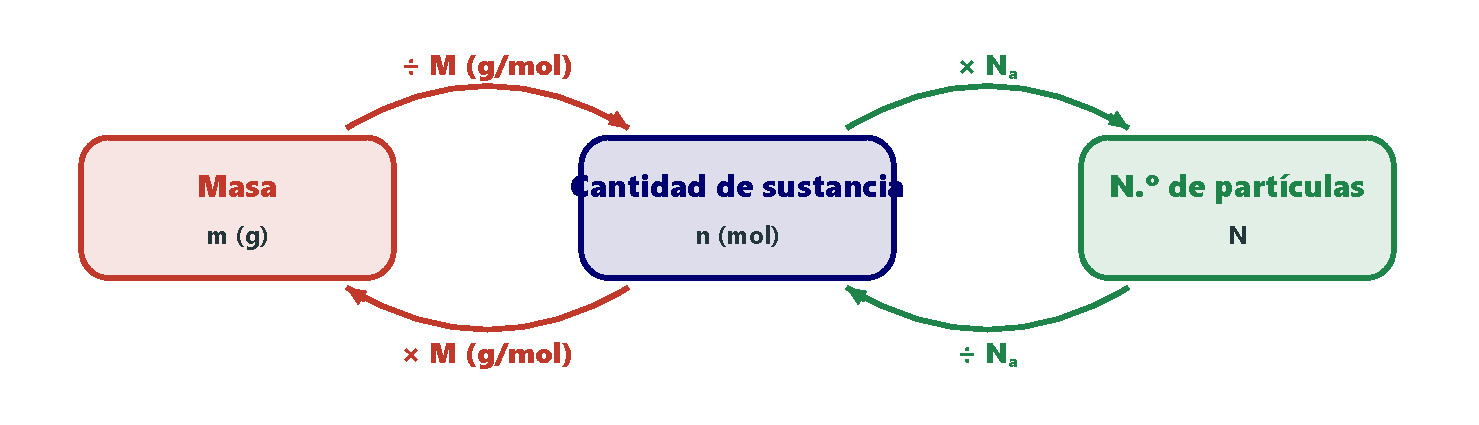
\includegraphics[width=0.85\textwidth]{images/UD3/mol_relaciones}
    \caption{Relación entre la masa, la cantidad de sustancia y el número de partículas.}
    \label{fig:mol_relaciones}
\end{figure}

\begin{example}
    \textbf{Algunos cálculos con el mol.}
    \begin{itemize}
        \item \textbf{¿Cuántos átomos hay en \qty{4}{\gram} de helio?} \(M(\ch{He}) = \qty{4}{\gram\per\mol}\); \(n = \frac{\qty{4}{\gram}}{\qty{4}{\gram\per\mol}} = \qty{1}{\mol}\); \(N = 1 \cdot \num{6.022e23} = \textcolor{red}{\num{6.022e23}}\) átomos.
        \item \textbf{¿Cuántas moléculas y átomos hay en \qty{2}{\mol} de cloro, \ch{Cl2}?} \(N = 2 \cdot \num{6.022e23} = \textcolor{red}{\num{1.2044e24}}\) moléculas, y el doble de átomos: \textcolor{red}{\num{2.4088e24}} átomos.
        \item \textbf{¿Qué masa tienen \num{1.2044e24} moléculas de agua?} \(n = \frac{\num{1.2044e24}}{\num{6.022e23}} = \qty{2}{\mol}\); \(m = n \cdot M = 2 \cdot 18 = \textcolor{red}{\qty{36}{\gram}}\).
        \item \textbf{¿Qué masa tienen \qty{1.5}{\mol} de \ch{HCl}?} \(m = \qty{1.5}{\mol} \cdot \qty{36.5}{\gram\per\mol} = \textcolor{red}{\qty{54.75}{\gram}}\).
        \item \textbf{¿Qué cantidad de sustancia hay en \qty{17}{\gram} de \ch{H2S}?} \(M = \qty{34}{\gram\per\mol}\); \(n = \frac{17}{34} = \textcolor{red}{\qty{0.5}{\mol}}\).
    \end{itemize}
\end{example}

\begin{exercise}
    Un frasco contiene \qty{63.5}{\gram} de yodo, \ch{I2}.
    \begin{enumerate}[label=\alph*)]
        \item ¿Qué cantidad de sustancia contiene?
        \item ¿Cuántas moléculas?
        \item ¿Cuántos átomos?
    \end{enumerate}
    \begin{solu}
        \textcolor{blue}{\(M(\ch{I2}) = 2 \cdot 127 = \qty{254}{\gram\per\mol}\).}
        a) \(n = \frac{\qty{63.5}{\gram}}{\qty{254}{\gram\per\mol}} = \textcolor{red}{\qty{0.25}{\mol}}\). b) \(N = \num{0.25} \cdot \num{6.022e23} = \textcolor{red}{\num{1.5055e23}}\) moléculas. c) \(2 \cdot \num{1.5055e23} = \textcolor{red}{\num{3.011e23}}\) átomos.
    \end{solu}
\end{exercise}

\begin{exercise}
    Un recipiente cerrado contiene \qty{16}{\gram} de dióxido de azufre, \ch{SO2}.
    \begin{enumerate}[label=\alph*)]
        \item ¿Cuál es la masa molar del \ch{SO2}?
        \item ¿Qué cantidad de sustancia contiene?
        \item ¿Cuántas moléculas hay?
        \item ¿Cuántos átomos de azufre y de oxígeno contiene?
    \end{enumerate}
    \begin{solu}
        a) \(M = 32 + 2 \cdot 16 = \textcolor{red}{\qty{64}{\gram\per\mol}}\). b) \(n = \frac{16}{64} = \textcolor{red}{\qty{0.25}{\mol}}\). c) \(N = \num{0.25} \cdot \num{6.022e23} = \textcolor{red}{\num{1.5055e23}}\) moléculas. d) Cada molécula tiene 1 átomo de S y 2 de O: \textcolor{red}{\num{1.5055e23}} átomos de S y \textcolor{red}{\num{3.011e23}} átomos de O.
    \end{solu}
\end{exercise}

\begin{exercise}
    Tienes \qty{8.8}{\gram} de \ch{CO2}.
    \begin{enumerate}[label=\alph*)]
        \item ¿Qué cantidad de sustancia hay en la muestra?
        \item ¿Cuántas moléculas contiene?
    \end{enumerate}
    \begin{solu}
        a) \(M(\ch{CO2}) = \qty{44}{\gram\per\mol}\); \(n = \frac{\num{8.8}}{44} = \textcolor{red}{\qty{0.2}{\mol}}\). b) \(N = \num{0.2} \cdot \num{6.022e23} = \textcolor{red}{\num{1.2044e23}}\) moléculas.
    \end{solu}
\end{exercise}

\begin{exercise}
    ¿Cuántos átomos hay en \qty{1}{\gram} de oro? ¿Cuál es la masa de un átomo de oro? ¿Y la de \num{3.011e24} átomos?
    \begin{solu}
        \textcolor{blue}{\(M(\ch{Au}) = \qty{197}{\gram\per\mol}\).}
        \(n = \frac{1}{197} = \qty{5.076e-3}{\mol}\); \(N = \num{5.076e-3} \cdot \num{6.022e23} = \textcolor{red}{\num{3.057e21}}\) átomos.
        Masa de un átomo: \(\dfrac{\qty{197}{\gram\per\mol}}{\qty{6.022e23}{\per\mol}} = \textcolor{red}{\qty{3.271e-22}{\gram}}\).
        \num{3.011e24} átomos son \(\frac{\num{3.011e24}}{\num{6.022e23}} = \qty{5}{\mol}\); \(m = 5 \cdot 197 = \textcolor{red}{\qty{985}{\gram}}\).
    \end{solu}
\end{exercise}

\begin{exercise}
    Calcula la masa de:
    \begin{enumerate}[label=\alph*)]
        \item \qty{0.25}{\mol} de átomos de cloro;
        \item \qty{0.25}{\mol} de moléculas de cloro, \ch{Cl2};
        \item \qty{2}{\mol} de átomos de oxígeno.
    \end{enumerate}
    \begin{solu}
        \textcolor{blue}{\(m = n \cdot M\):}
        a) \(\num{0.25} \cdot \num{35.5} = \textcolor{red}{\qty{8.875}{\gram}}\). b) \(\num{0.25} \cdot 71 = \textcolor{red}{\qty{17.75}{\gram}}\). c) \(2 \cdot 16 = \textcolor{red}{\qty{32}{\gram}}\) (que es la masa de \qty{1}{\mol} de moléculas \ch{O2}).
    \end{solu}
\end{exercise}

\begin{exercise}
    En una muestra de \qty{5.6}{\gram} de nitrógeno gaseoso, \ch{N2}, calcula:
    \begin{enumerate}[label=\alph*)]
        \item la cantidad de sustancia;
        \item el número de moléculas;
        \item el número de átomos.
    \end{enumerate}
    \begin{solu}
        a) \(n = \frac{\qty{5.6}{\gram}}{\qty{28}{\gram\per\mol}} = \textcolor{red}{\qty{0.2}{\mol}}\). b) \(N = \num{0.2} \cdot \num{6.022e23} = \textcolor{red}{\num{1.2044e23}}\) moléculas. c) \(2 \cdot \num{1.2044e23} = \textcolor{red}{\num{2.4088e23}}\) átomos.
    \end{solu}
\end{exercise}

\begin{exercise}
    ¿Cuál de estas muestras contiene más moléculas?
    \begin{enumerate}[label=\alph*)]
        \item \qty{10}{\gram} de agua, \ch{H2O};
        \item \qty{10}{\gram} de oxígeno, \ch{O2};
        \item \qty{10}{\gram} de hidrógeno, \ch{H2}.
    \end{enumerate}
    \begin{solu}
        \textcolor{blue}{Tendrá más moléculas la que tenga más moles:}
        a) \(n = \frac{10}{18} = \qty{0.56}{\mol}\). b) \(n = \frac{10}{32} = \qty{0.31}{\mol}\). c) \(n = \frac{10}{2} = \qty{5}{\mol}\). Tiene más moléculas el \textcolor{red}{hidrógeno}.
    \end{solu}
\end{exercise}

\begin{exercise}
    Calcula el número de moléculas que hay en:
    \begin{enumerate}[label=\alph*)]
        \item \qty{0.25}{\mol} de \ch{NH3};
        \item \qty{1.5}{\mol} de \ch{O2};
        \item \qty{36}{\gram} de agua;
        \item \qty{73}{\gram} de \ch{HCl}.
    \end{enumerate}
    \begin{solu}
        a) \(N = \num{0.25} \cdot \num{6.022e23} = \textcolor{red}{\num{1.5055e23}}\). b) \(N = \num{1.5} \cdot \num{6.022e23} = \textcolor{red}{\num{9.033e23}}\). c) \(n = \frac{36}{18} = \qty{2}{\mol}\); \(N = \textcolor{red}{\num{1.2044e24}}\). d) \(n = \frac{73}{\num{36.5}} = \qty{2}{\mol}\); \(N = \textcolor{red}{\num{1.2044e24}}\).
    \end{solu}
\end{exercise}

\begin{exercise}
    Calcula la masa de:
    \begin{enumerate}[label=\alph*)]
        \item \qty{0.5}{\mol} de \ch{HCl};
        \item \qty{2}{\mol} de \ch{CO2};
        \item \num{1.2044e22} moléculas de \ch{CH4};
        \item \num{1.5055e24} moléculas de \ch{NH3}.
    \end{enumerate}
    \begin{solu}
        a) \(m = \num{0.5} \cdot \num{36.5} = \textcolor{red}{\qty{18.25}{\gram}}\). b) \(m = 2 \cdot 44 = \textcolor{red}{\qty{88}{\gram}}\).
        c) \(n = \frac{\num{1.2044e22}}{\num{6.022e23}} = \qty{0.02}{\mol}\); \(m = \num{0.02} \cdot 16 = \textcolor{red}{\qty{0.32}{\gram}}\).
        d) \(n = \frac{\num{1.5055e24}}{\num{6.022e23}} = \qty{2.5}{\mol}\); \(m = \num{2.5} \cdot 17 = \textcolor{red}{\qty{42.5}{\gram}}\).
    \end{solu}
\end{exercise}
